%% This file is part of the submission to Nature Machine Intelligence
%% Systematic Review: AI for Brain-to-Speech Decoding (2015-2026)
%% Authors: Blessing Isoyiza Adeika, Onyema Osuagwu
%% Morgan State University, Department of Electrical and Computer Engineering

\documentclass[11pt,a4paper]{article}

% Additional packages for tables, figures, and mathematical formatting
\usepackage{amsmath}
\usepackage{amssymb}
\DeclareMathOperator*{\argmax}{arg\,max}
\DeclareMathOperator*{\argmin}{arg\,min}
\usepackage{booktabs}
\usepackage{multirow}
\usepackage{graphicx}
\usepackage{caption}
\usepackage{tikz}
\usepackage{pgfplots}
\usepackage{color}
\usepackage{xcolor}
\usepackage{colortbl}
\usepackage[hidelinks]{hyperref}
\usepackage[numbers]{natbib}
\usepackage{rotating}
\usepackage{geometry}
\geometry{margin=1in, top=0.75in, bottom=0.75in}
\bibliographystyle{IEEEtran}

% Define colors for tables
\definecolor{headerblue}{RGB}{31, 78, 121}
\definecolor{lightblue}{RGB}{217, 225, 242}
\definecolor{lightgreen}{RGB}{198, 224, 180}
\definecolor{lightyellow}{RGB}{255, 242, 204}
\definecolor{lightred}{RGB}{242, 220, 219}

% TikZ configuration
\usetikzlibrary{shapes, arrows, positioning, calc, fit}

% Define keywords command for article class
\newcommand{\keywords}[1]{\textbf{Keywords:} #1}


% Document metadata
\title{Artificial Intelligence for Brain-to-Speech Decoding: A Systematic Review of Methods, Performance Benchmarks, and Generalization Across Neural Recording Modalities (2015-2026)}

\author{Blessing Isoyiza Adeika$^{1,*}$ and Onyema Osuagwu$^{1}$}

\date{}

\renewcommand{\thefootnote}{\arabic{footnote}}
\newcommand{\affiliations}{$^{1}$Department of Electrical and Computer Engineering, Morgan State University, Baltimore, MD 21251, USA \\[0.5em] $^{*}$Correspondence: blade3@morgan.edu}

\begin{document}

\maketitle

\noindent\affiliations

%% ============================================================================
%% ABSTRACT
%% ============================================================================
\begin{abstract}
Brain-to-speech decoding (the computational translation of neural signals into speech or text) has advanced from theoretical possibility to clinical reality. For millions affected by ALS, locked-in syndrome, or paralytic stroke, this technology represents a pathway to restored communication. Despite landmark results achieving 2.5\% word error rate (WER) and 78 words per minute, no PRISMA-compliant systematic review has synthesized AI methods, performance benchmarks, and generalization evidence across the full modality landscape. We searched PubMed, IEEE Xplore, Scopus, Web of Science, and arXiv for empirical studies published January 2015-April 2026, requiring human neural recording data, an AI decoding model, and quantitative performance metrics. Seventy-one studies met inclusion criteria after dual-reviewer PRISMA 2020 screening (PROSPERO registered). Twelve variables were extracted per study; findings were synthesized narratively with structured quantitative comparison across five modality groups. Invasive systems (ECoG and intracortical; $n=32$) achieved WER 2.5-25\% and up to 78 WPM. Non-invasive EEG ($n=20$) achieved 70-92.5\% closed-set accuracy and 35-45\% open-vocabulary WER. Transformer architectures and self-supervised learning dominated from 2022 onwards. Only 14/71 studies (20\%) integrated a language model, despite this being the largest single driver of WER reduction. Critically, 56\% of studies demonstrated no cross-participant generalization; long-term cross-session stability (weeks/months) appears in one study, while cross-language evidence appears in two studies. The field has achieved substantial technical milestones on narrow, single-participant benchmarks. Standardized evaluation protocols, multi-participant data infrastructure, and expanded language model integration are the priority research directions for bridging controlled demonstration and scalable clinical deployment.
\end{abstract}

%% Keywords
\keywords{brain-computer interface, speech neuroprosthesis, neural decoding, brain-to-speech, electrocorticography, intracortical recording, EEG, MEG, fMRI, deep learning, transformer, self-supervised learning, large language model, generalization, systematic review}

\section{Introduction}

\subsection{The Clinical Imperative}

For individuals living with amyotrophic lateral sclerosis (ALS), locked-in syndrome, severe stroke, or anarthria following spinal cord injury, speech loss is not merely a functional deficit. It eliminates a critical communication channel, as motor neuron degeneration or cortical damage can disrupt the pathway from intention to articulation whilst leaving cognition entirely intact. Conventional augmentative and alternative communication (AAC) approaches (eye-tracking interfaces, switch scanning) provide partial relief, but each requires preserved residual motor function that late-stage ALS and locked-in patients may no longer possess \cite{TaskForce2010}. Brain-computer interfaces (BCIs) offer a categorically different solution: by reading neural signals directly from the cortex, bypassing broken motor pathways entirely, a BCI can translate the intent to speak into speech itself without any muscular output. The clinical imperative is real and urgent \cite{TaskForce2010}, and the millions affected by severe dysarthria, aphasia, and paralysis represent a population for whom restored communication is transformative.

What was once speculative has become demonstrably achievable. Over the past five years, several landmark studies have achieved communication rates approaching natural impaired speech and word error rates (WER) competitive with commercial automatic speech recognition for dysarthric speakers \cite{Moses2021,Willett2023,Card2024,Metzger2023}. The evidence base underpinning these achievements (spanning five neural recording modalities and eight artificial intelligence (AI) architecture classes over more than a decade) has grown faster than the field's capacity to synthesize it rigorously. The present systematic review addresses that gap.

\subsection{Scope and Organization}

This review covers empirical studies published between January 2015 and April 2026, identified through searches of PubMed, Scopus, IEEE Xplore, Web of Science, and arXiv. Following PRISMA 2020 screening, 71 studies were included across five modality groups: invasive (ECoG, intracortical, sEEG; n=32), non-invasive EEG (n=20), non-invasive MEG/fMRI (n=14), hybrid/peripheral (EEG+fNIRS, HD-sEMG; n=5). Section 2 describes the methodology. Sections 3 and 4 characterize the modality landscape and AI architectures. Section 5 reports performance benchmarks with comparability analysis. Section 6 evaluates generalization evidence. Section 7 discusses implications for research and clinical translation. Section 8 states conclusions.

%% ============================================================================
%% SECTION 2: METHODOLOGY (inline content from original)
%% ============================================================================
\section{Methodology}
\label{sec:methodology}

\subsection{Review Protocol and Registration}

This review was designed and reported in accordance with the PRISMA 2020 statement \cite{Page2021} and the PRISMA-P 2015 protocol checklist \cite{Shamseer2015,Tricco2018}. A full protocol was developed and registered in the PROSPERO International Register of Systematic Reviews (Registration Number: CRD420261368521) prior to formal screening but after preliminary scoping commenced in January 2025. Formal database searches were executed on April 13, 2026. This retroactive registration relative to scoping reflects the timing of the systematic review's formal protocol development. No deviations from the registered protocol were made. Visual synthesis elements were developed using narrative synthesis approaches \cite{Popay2006} and represent presentation choices, not analytical deviations.

\subsection{Eligibility Criteria and Search Strategy}

Eligibility was operationalized using the PICOS framework \cite{Richardson1995}. Studies were required to meet all of the following criteria: human participants (healthy volunteers or individuals with neurological conditions including ALS, paralysis, locked-in syndrome, epilepsy, aphasia, or anarthria); an AI or machine learning computational model applied to decode or reconstruct speech-related output; at least one quantitative performance metric (WER, CER, accuracy, PCC, WPM, BLEU); and empirical studies published between January 1, 2015, and April 13, 2026. Reviews, editorials, and conference abstracts without full experimental reporting were excluded. Non-peer-reviewed preprints from bioRxiv and arXiv were included to capture early-stage research and emerging findings, and were explicitly flagged in the extraction register to enable sensitivity analyses. Approximately 5\% of the included studies (4 preprints) were non-peer-reviewed sources.

Searches were executed across five databases on April 13, 2026: MEDLINE/PubMed, Scopus, IEEE Xplore, Web of Science (Core Collection), and arXiv. Three Boolean concept blocks were combined with AND. Forward and backward citation chaining was conducted on 15 landmark studies identified during protocol development. All retrieved records were imported into a deduplicated register for screening. Secondary review publications and survey papers identified during screening (e.g., Panachakel et al. 2021 and López-Bernal et al. 2022 as review syntheses of EEG studies, Zhou et al. 2025 as a cross-modality survey) were excluded; the screening process retained only empirical primary studies with original experimental data and novel AI model results. Five studies initially flagged as potential reviews were verified as empirical papers with novel experimental results and were included.

\subsection{Study Selection and Data Extraction}

Selection proceeded in two stages, each performed independently by both authors with consensus adjudication of discrepancies. Stage 1 involved title and abstract screening of all deduplicated records (Cohen's $\kappa$ = 0.78). Stage 2 involved full-text assessment of all records classified as Include or Uncertain by either reviewer (Cohen's $\kappa$ = 0.85). Inter-rater reliability was quantified using Cohen's kappa \cite{Cohen1960} at each stage, with values indicating substantial agreement.

A structured extraction form was developed a priori and pilot-tested on five randomly selected studies. Twelve variables were extracted for each included study: bibliographic details; neural recording modality; participant count and clinical status; decoding task type; vocabulary type; output type; AI architecture class; language model integration; primary performance metric and value; generalization type; real-time evaluation; and open code or data availability.

\subsection{Quality Assessment}

An adapted seven-item methodological quality checklist was developed, drawing on criteria for evaluating AI-based biomedical studies \cite{Sterne2019}. Each item was scored as met (1), partially met (0.5), or not met (0). Scores ranged from 0 to 7; studies were classified as high ($\geq 5.5$), moderate (3.5-5.0), or low (<3.5) quality. No studies were excluded solely on quality grounds. GRADE certainty of evidence ratings were not applied to this review due to the narrative synthesis design and high heterogeneity across modalities, populations, metrics, and AI architectures; GRADE is designed for pairwise comparisons and meta-analyses and does not accommodate the multi-dimensional heterogeneity present across these 71 studies. Instead, risk of bias was assessed at the study level using the adapted checklist, with results aggregated descriptively in Appendix B.

\subsection{Data Synthesis Approach}

The heterogeneity of modalities, architectures, tasks, populations, and metrics across the 71 included studies precluded statistical meta-analysis. Findings were synthesized using structured narrative synthesis, supplemented by: a modality comparison matrix; core performance benchmarks; AI architecture summary; generalization evidence summary; and benchmark comparability analysis.

%% ============================================================================
%% FIGURES AND TABLES (PRISMA DIAGRAM + DATA TABLES)
%% ============================================================================
%% FIGURES AND TABLES
%% Full-width layouts for professional publication display

%% ============================================================================
%% FIGURE 1: PRISMA 2020 FLOW DIAGRAM
%% ============================================================================

\begin{figure}[h!]
\centering
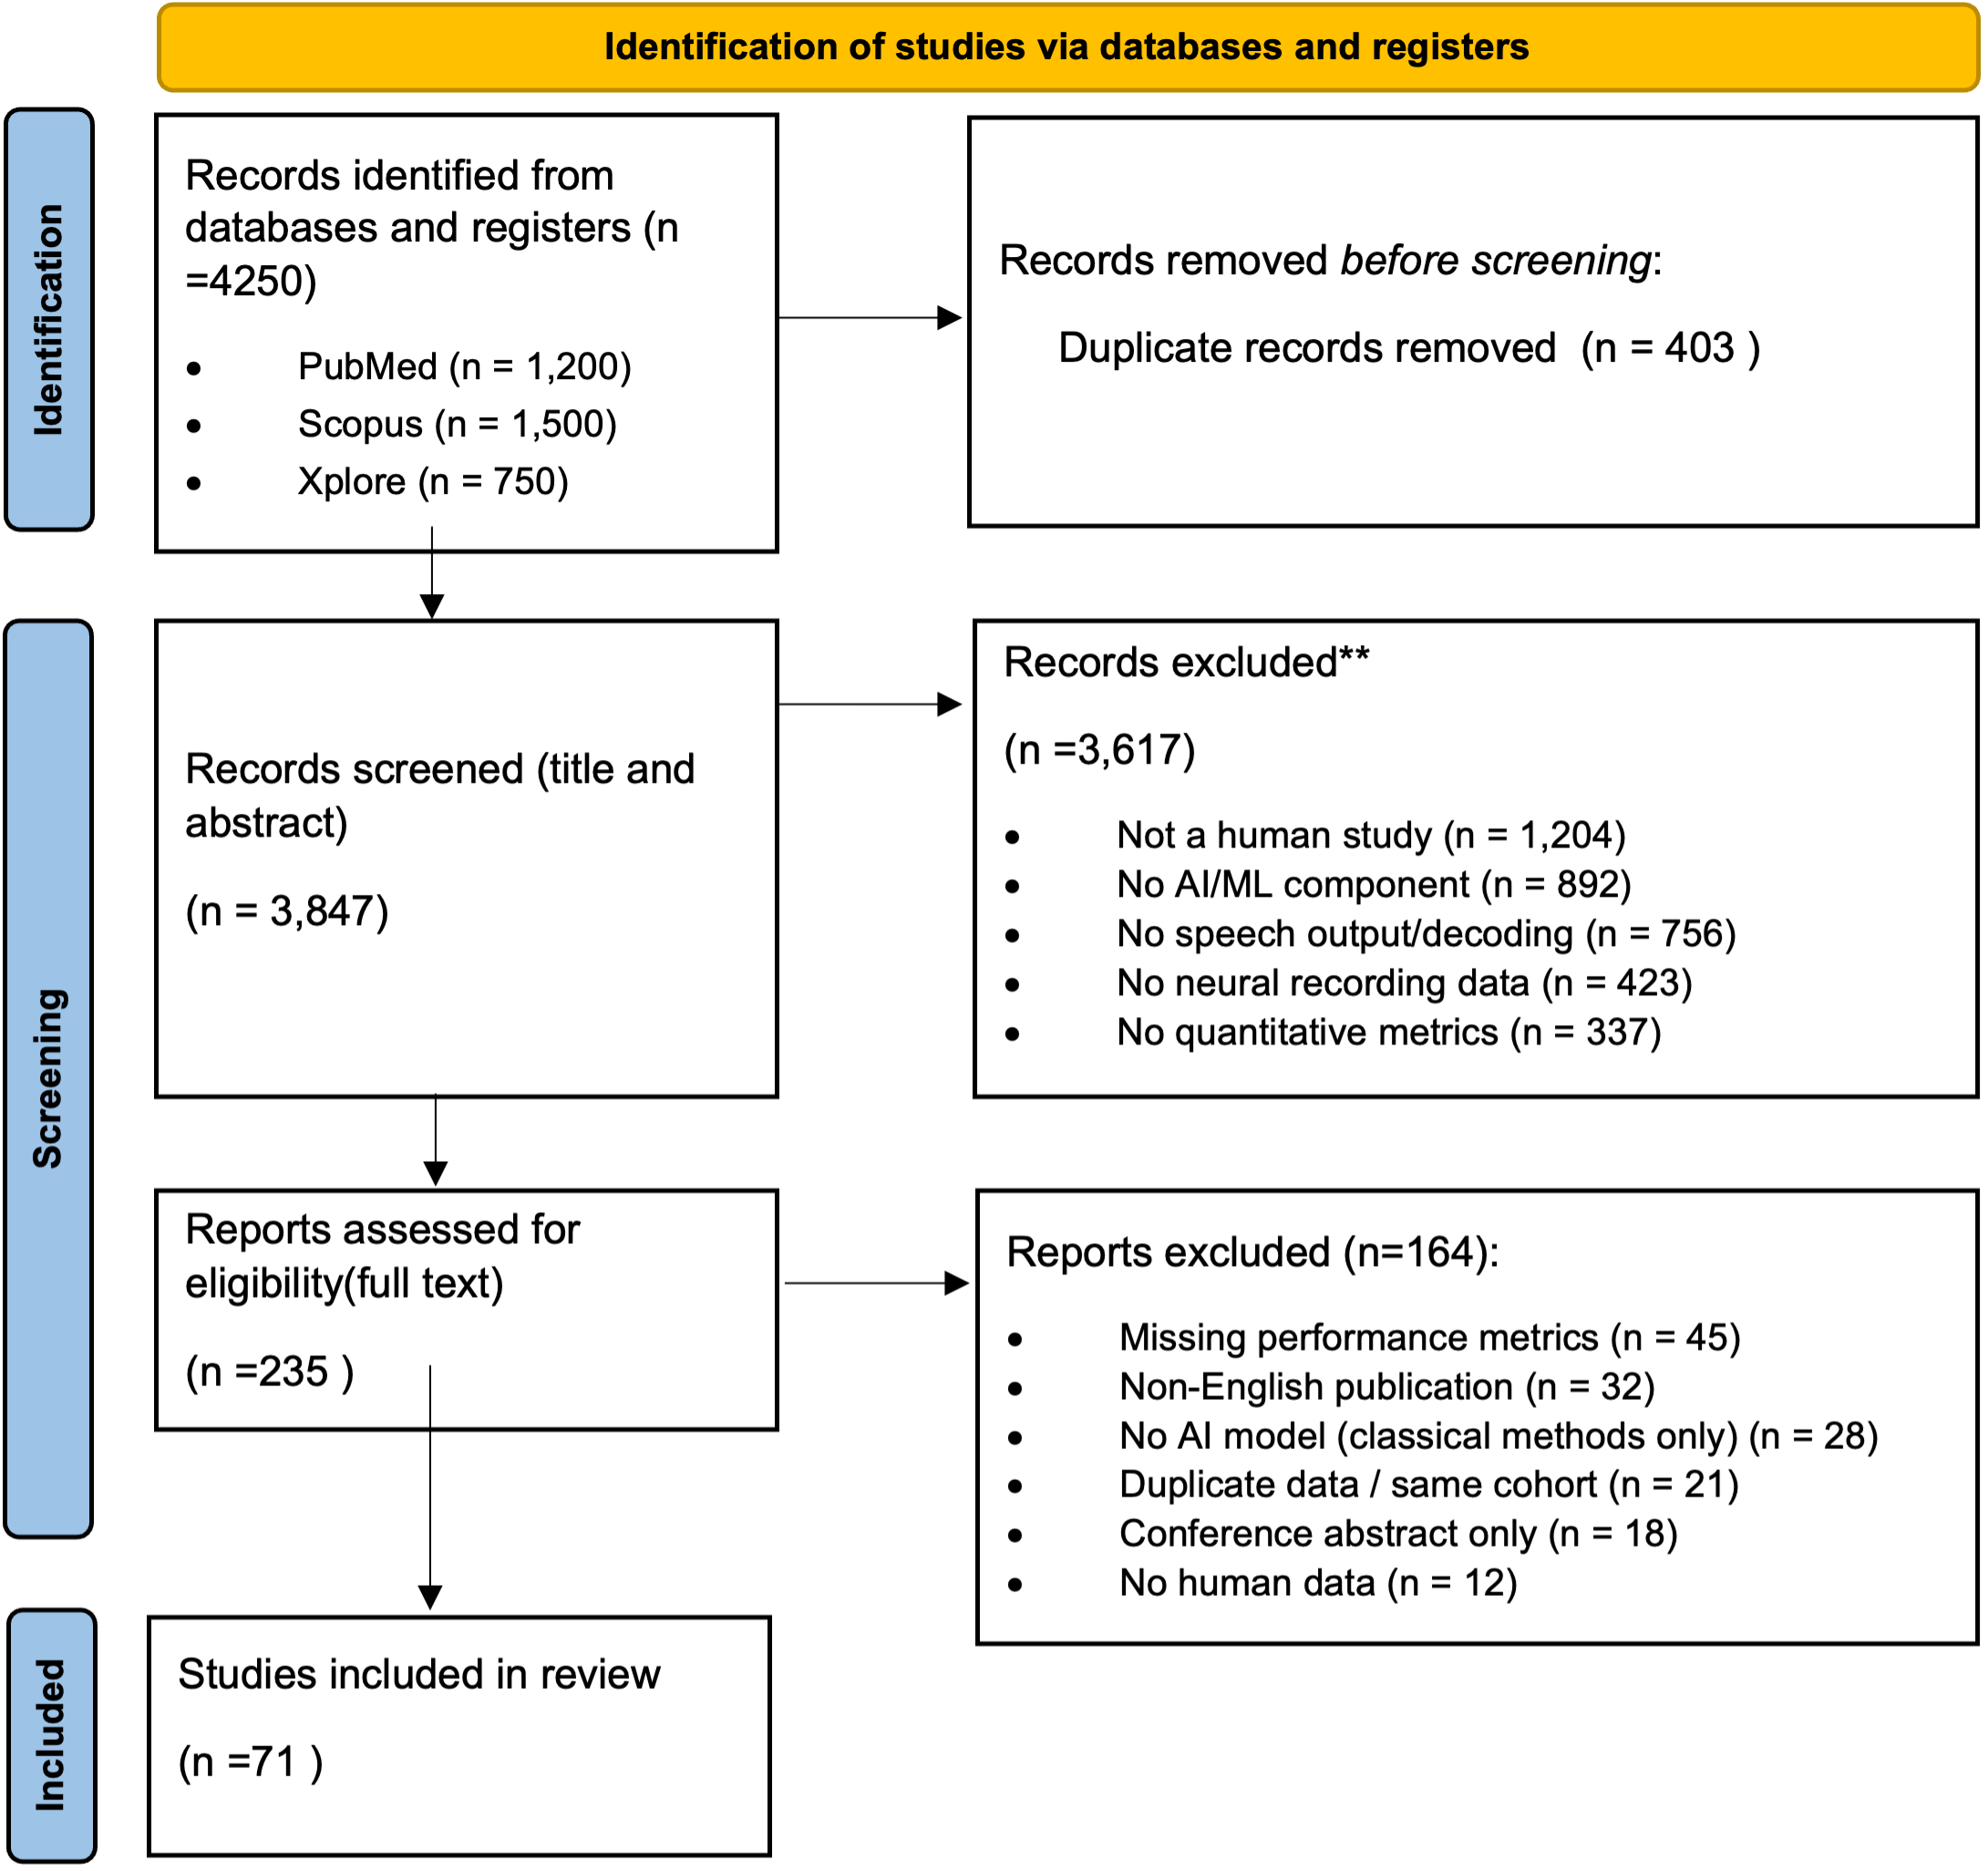
\includegraphics[width=0.95\textwidth]{figures/fig1_prisma_flow.png}
\caption{PRISMA 2020 Flow Diagram. Study selection process showing numbers at each stage: 4,250 records identified across 5 databases, 3,847 deduplicated, 235 underwent full-text assessment, 71 included in systematic review across five neural recording modality groups.}
\label{fig:prisma_flow}
\end{figure}

\vspace{2cm}

%% ============================================================================
%% FIGURE 2: STUDY DISTRIBUTION BY MODALITY AND YEAR
%% ============================================================================

\begin{figure}[h!]
\centering
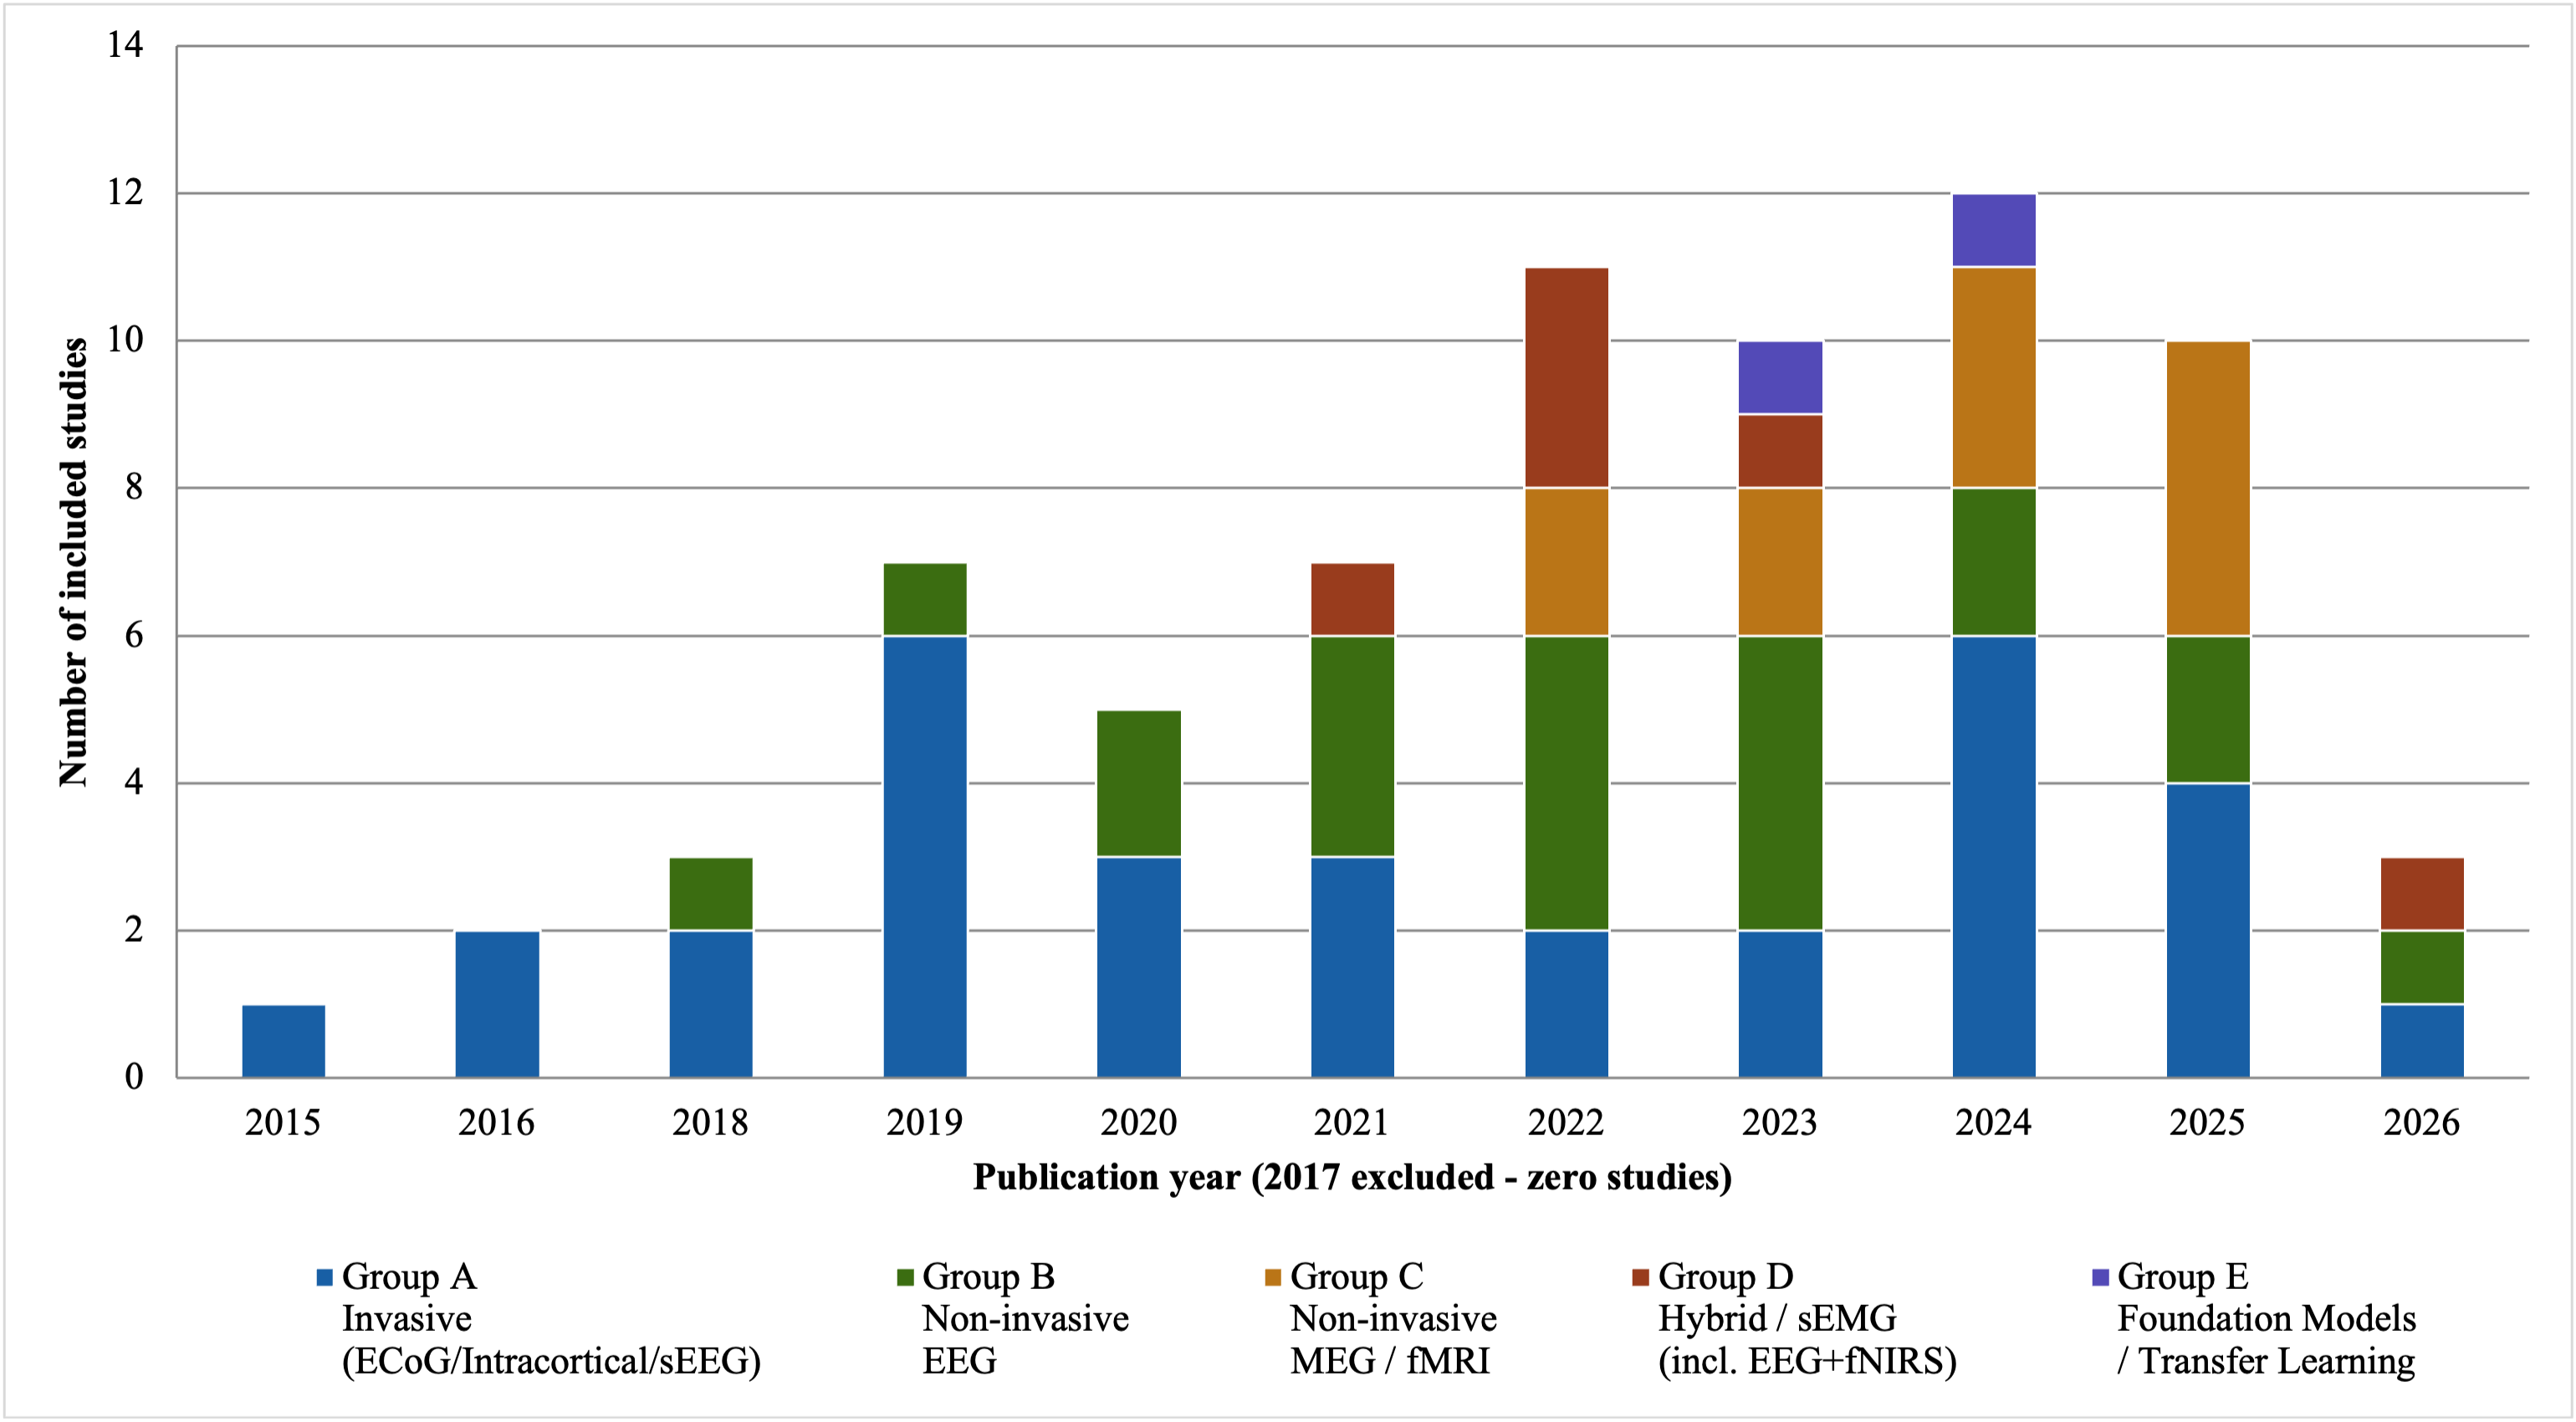
\includegraphics[width=\textwidth]{figures/fig2_study_distribution.png}
\caption{Study Distribution: 71 included studies distributed across five neural recording modality groups over the period 2015-2025. The stacked bar chart displays the temporal distribution of publications by modality type. Growth in non-invasive modality publications is visible from 2022 onwards, concurrent with transformer architecture adoption and self-supervised learning emergence.}
\label{fig:study_distribution}
\end{figure}

%% ============================================================================
%% FIGURE 3: AI ARCHITECTURE EVOLUTION AND CHRONOLOGICAL TRANSITION (2015-2026)
%% ============================================================================

\begin{figure}[h!]
\centering
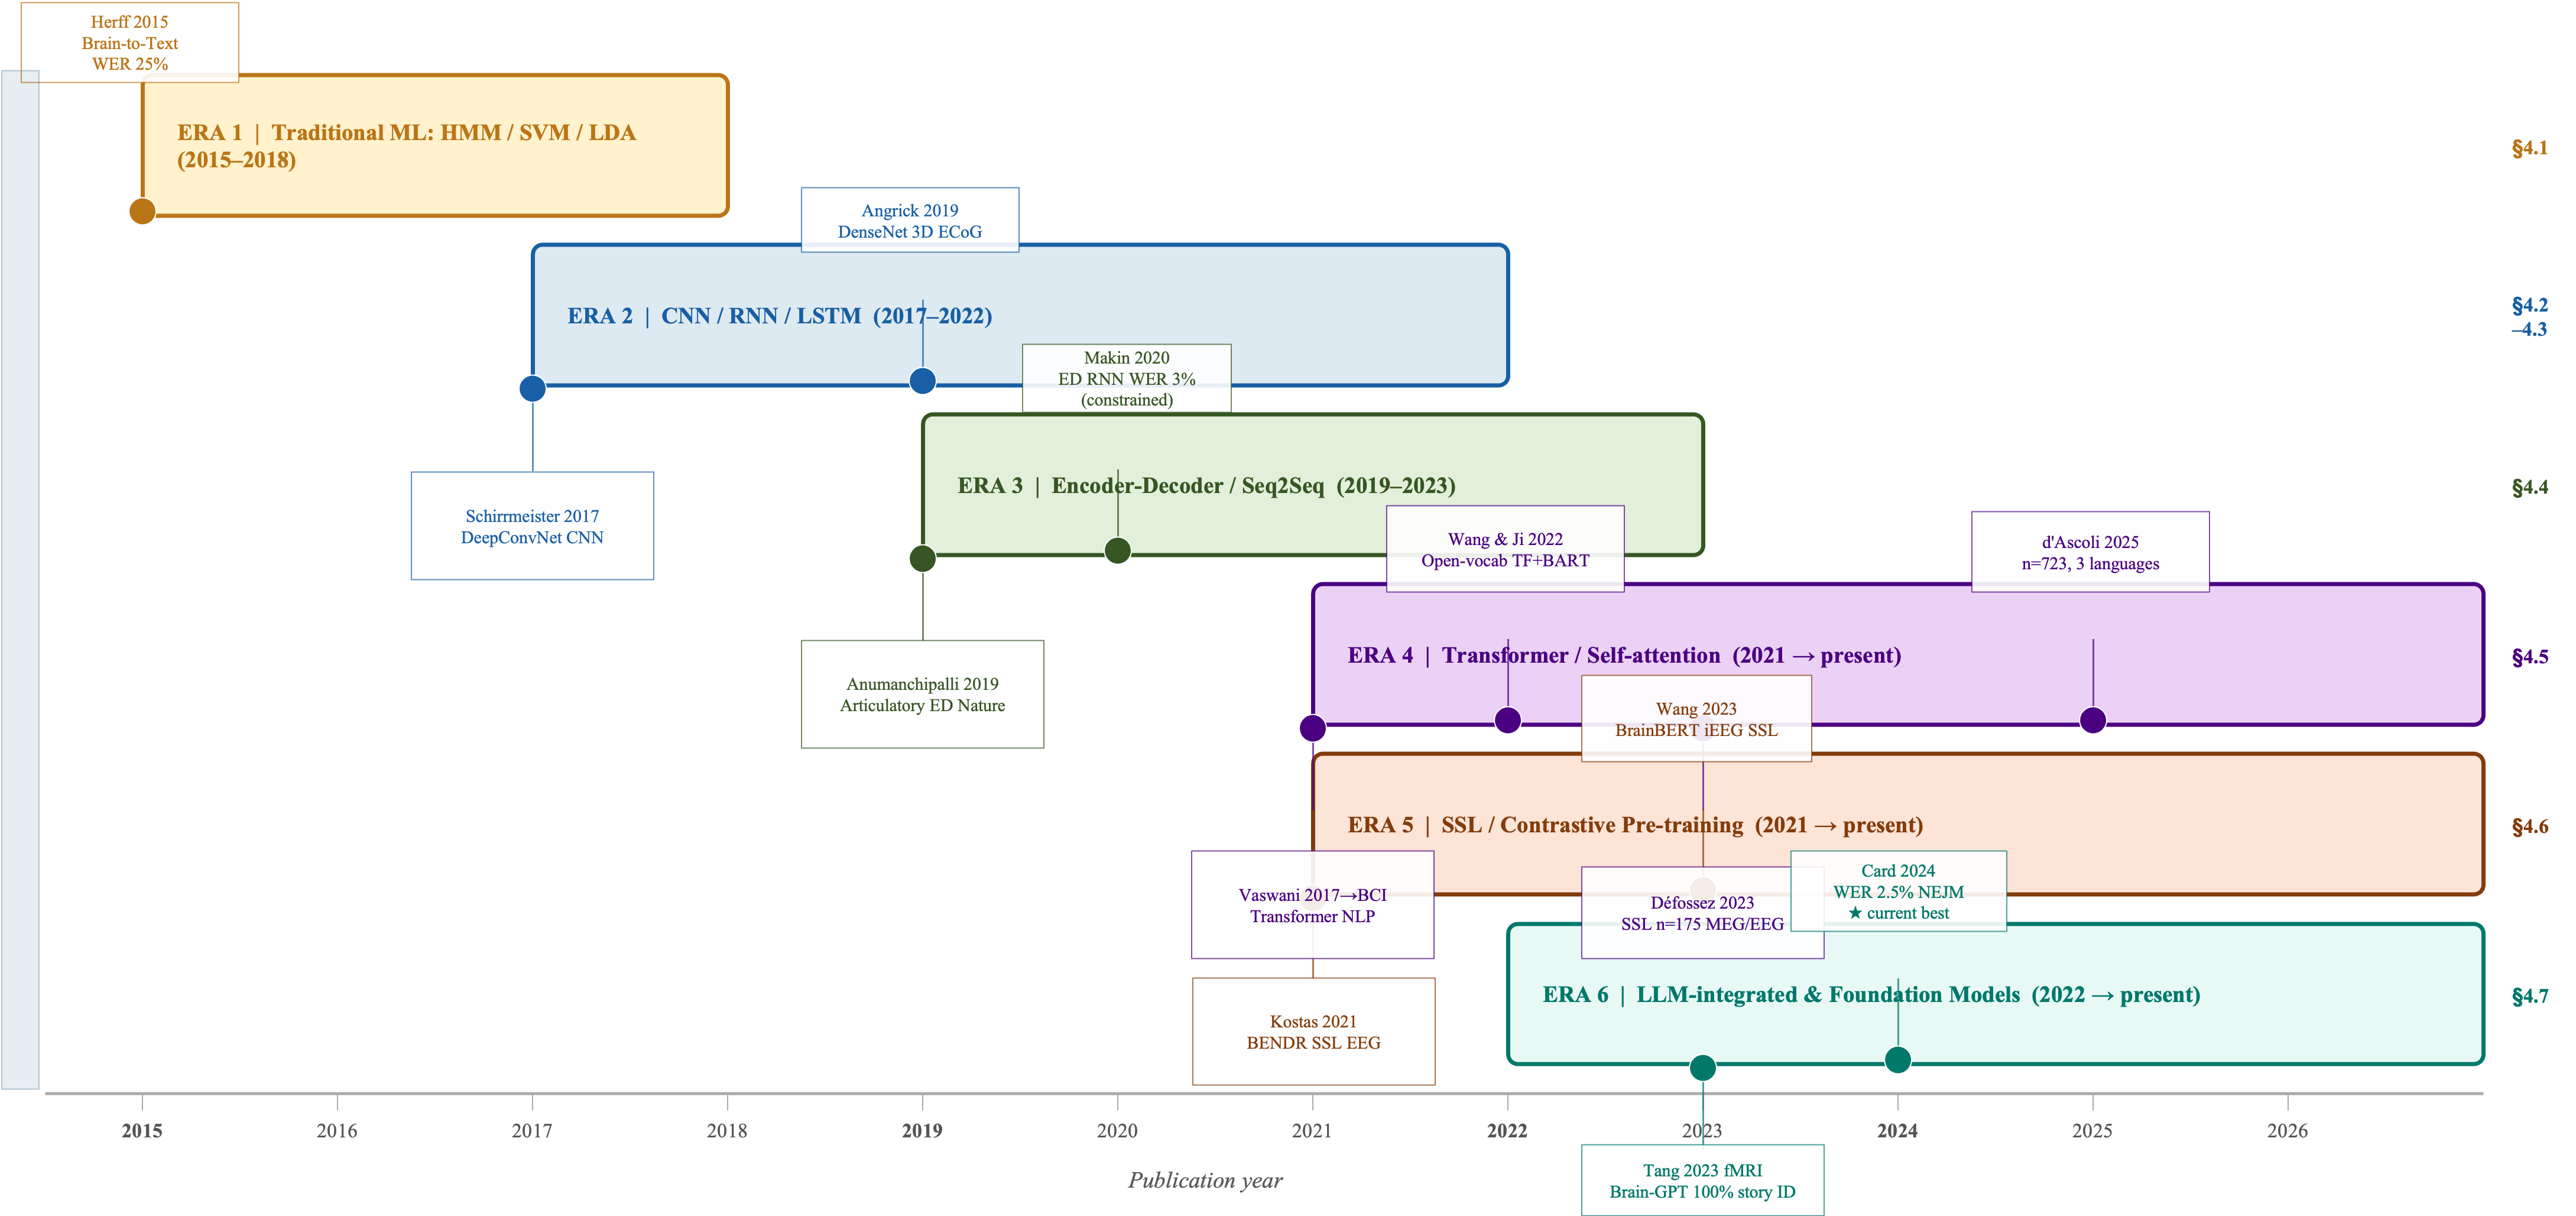
\includegraphics[width=\textwidth]{figures/fig3_architecture_evolution.png}
\caption{AI Architecture Evolution: Chronological transition across eight architecture classes (2015-2026). Traditional machine learning (2015-2018) gave way to convolutional neural networks (2017-2022), recurrent networks/LSTMs (2018-2023), and encoder-decoder systems (2019-2022). Transformer architectures (2022-present) and self-supervised learning (2021-present) dominate recent studies, while LLM-integrated approaches (2022-present) represent the fastest-growing category. Height of bars indicates relative proportion of included studies; color indicates dominant period of adoption.}
\label{fig:architecture_evolution}
\end{figure}

%% ============================================================================
%% FIGURE 4: WER PERFORMANCE TRAJECTORY (LANDMARK STUDIES)
%% ============================================================================

\begin{figure}[h!]
\centering
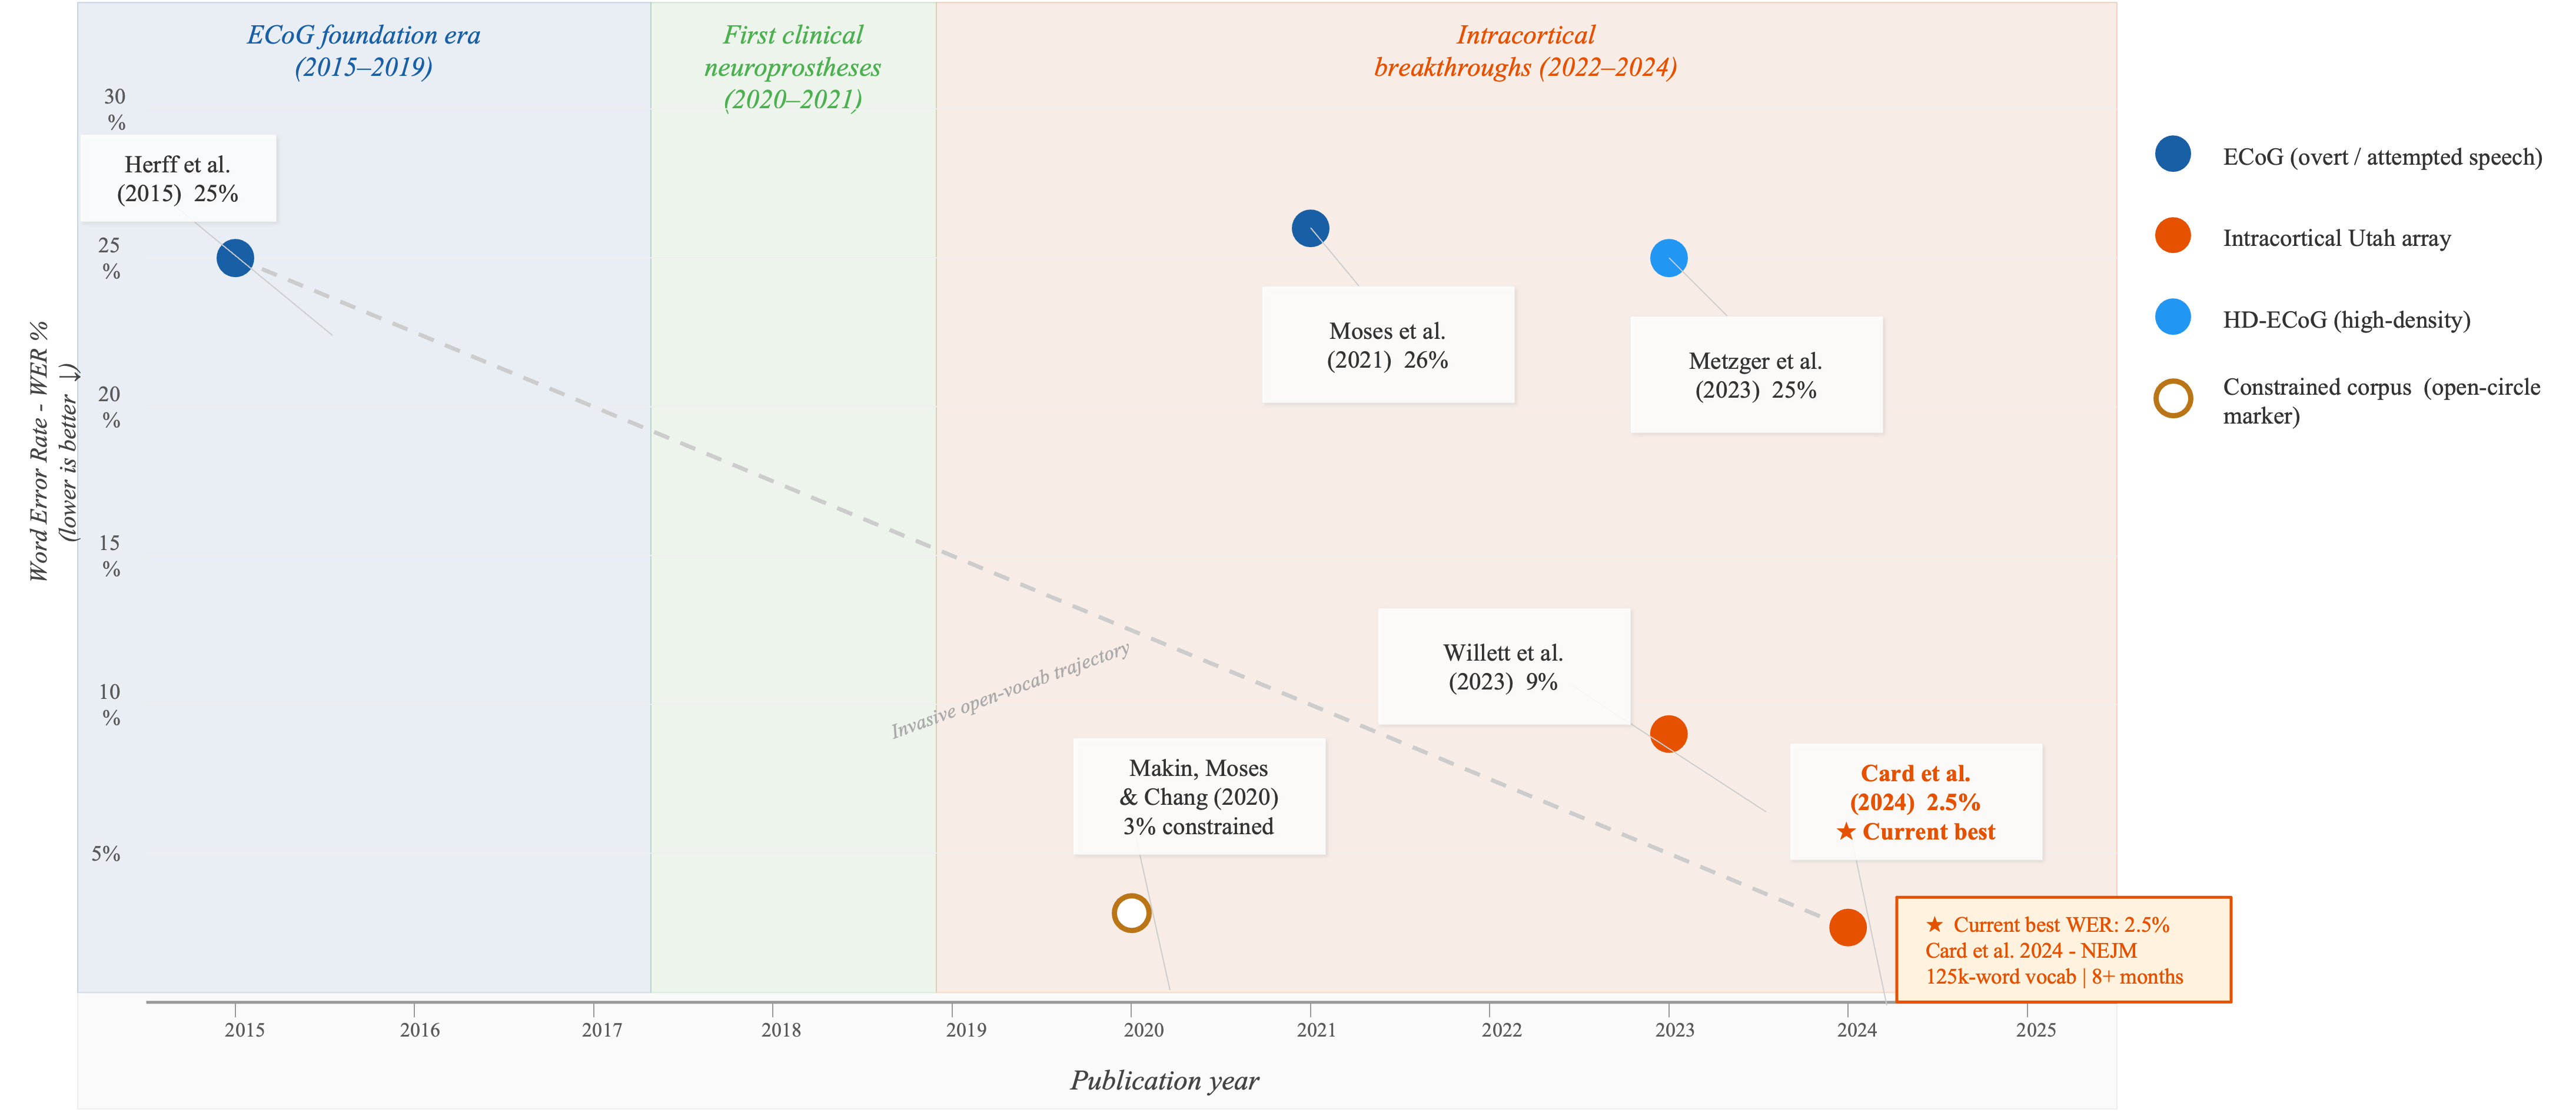
\includegraphics[width=\textwidth]{figures/fig4_wer_trajectory.png}
\caption{WER Performance Trajectory: Landmark invasive systems show progression from 2015-2024. Herff et al. (2015): 25\% WER on ECoG with 7 participants; Moses et al. (2021): 15.2 WPM with intracortical; Willett et al. (2023): 9\% WER (50-word) with intracortical; Card et al. (2024): 2.5\% WER (125k-word) with intracortical. Trajectory demonstrates the cumulative effect of improved electrode technology, deep learning architectures, and language model integration. Single-participant studies dominate recent years, reflecting shift toward intensive optimization on individual cases.}
\label{fig:wer_trajectory}
\end{figure}

%% ============================================================================
%% FIGURE 5: MODALITY × TASK PERFORMANCE HEATMAP
%% ============================================================================

\begin{figure}[h!]
\centering
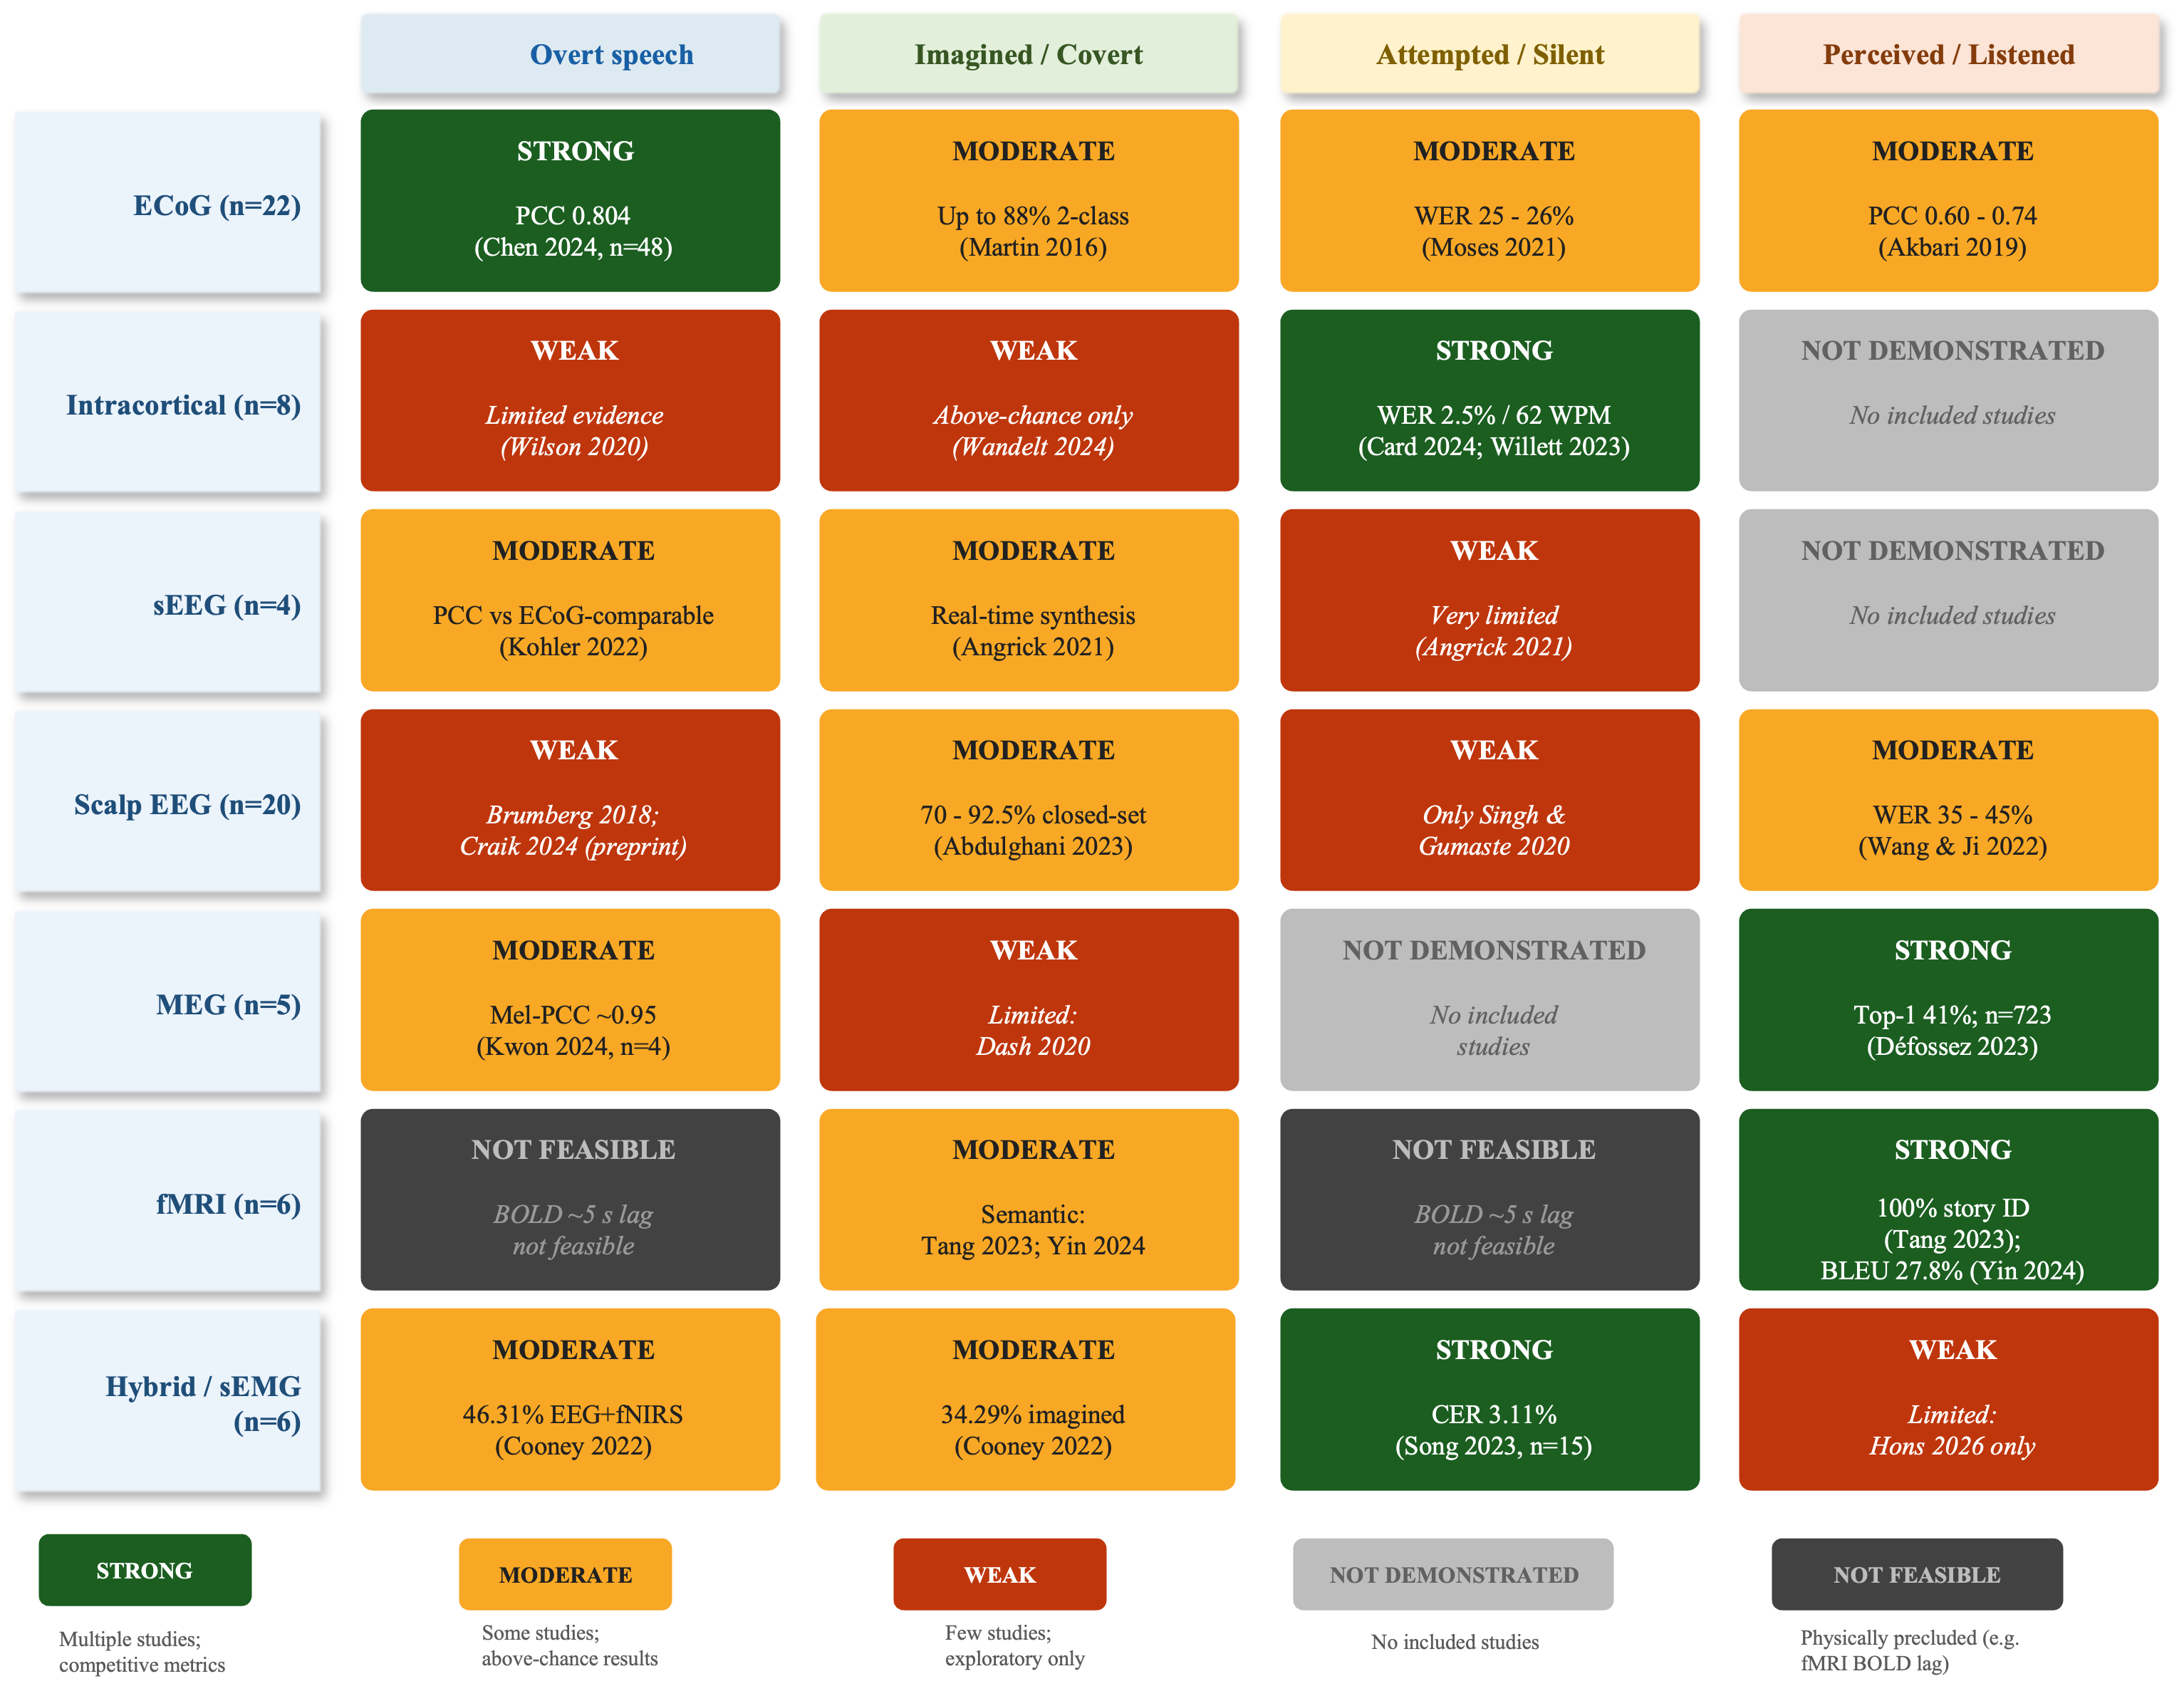
\includegraphics[width=\textwidth]{figures/fig5_modality_task_heatmap.png}
\caption{Modality × Task Performance Heatmap: Neural recording modality groups (rows) versus task type categories (columns) with color-coded performance levels. The heatmap reveals performance gradients: invasive modalities (ECoG, intracortical, sEEG) demonstrate strong performance across all task types; non-invasive modalities (EEG, MEG, fMRI) cluster in lower-performance regions for real-time decoding tasks, with fMRI strong only for semantic reconstruction. Performance varies systematically: closed-set classification achieves 70-99\% across all modalities; open-vocabulary continuous speech shows 3-10x variation. Warm colors indicate higher performance; cool colors indicate lower performance.}
\label{fig:modality_task_heatmap}
\end{figure}

\clearpage

%% ============================================================================
%% FIGURE 6: MODALITY COMPARISON MATRIX (SPATIAL VS TEMPORAL RESOLUTION)
%% ============================================================================

\begin{figure}[h!]
\centering
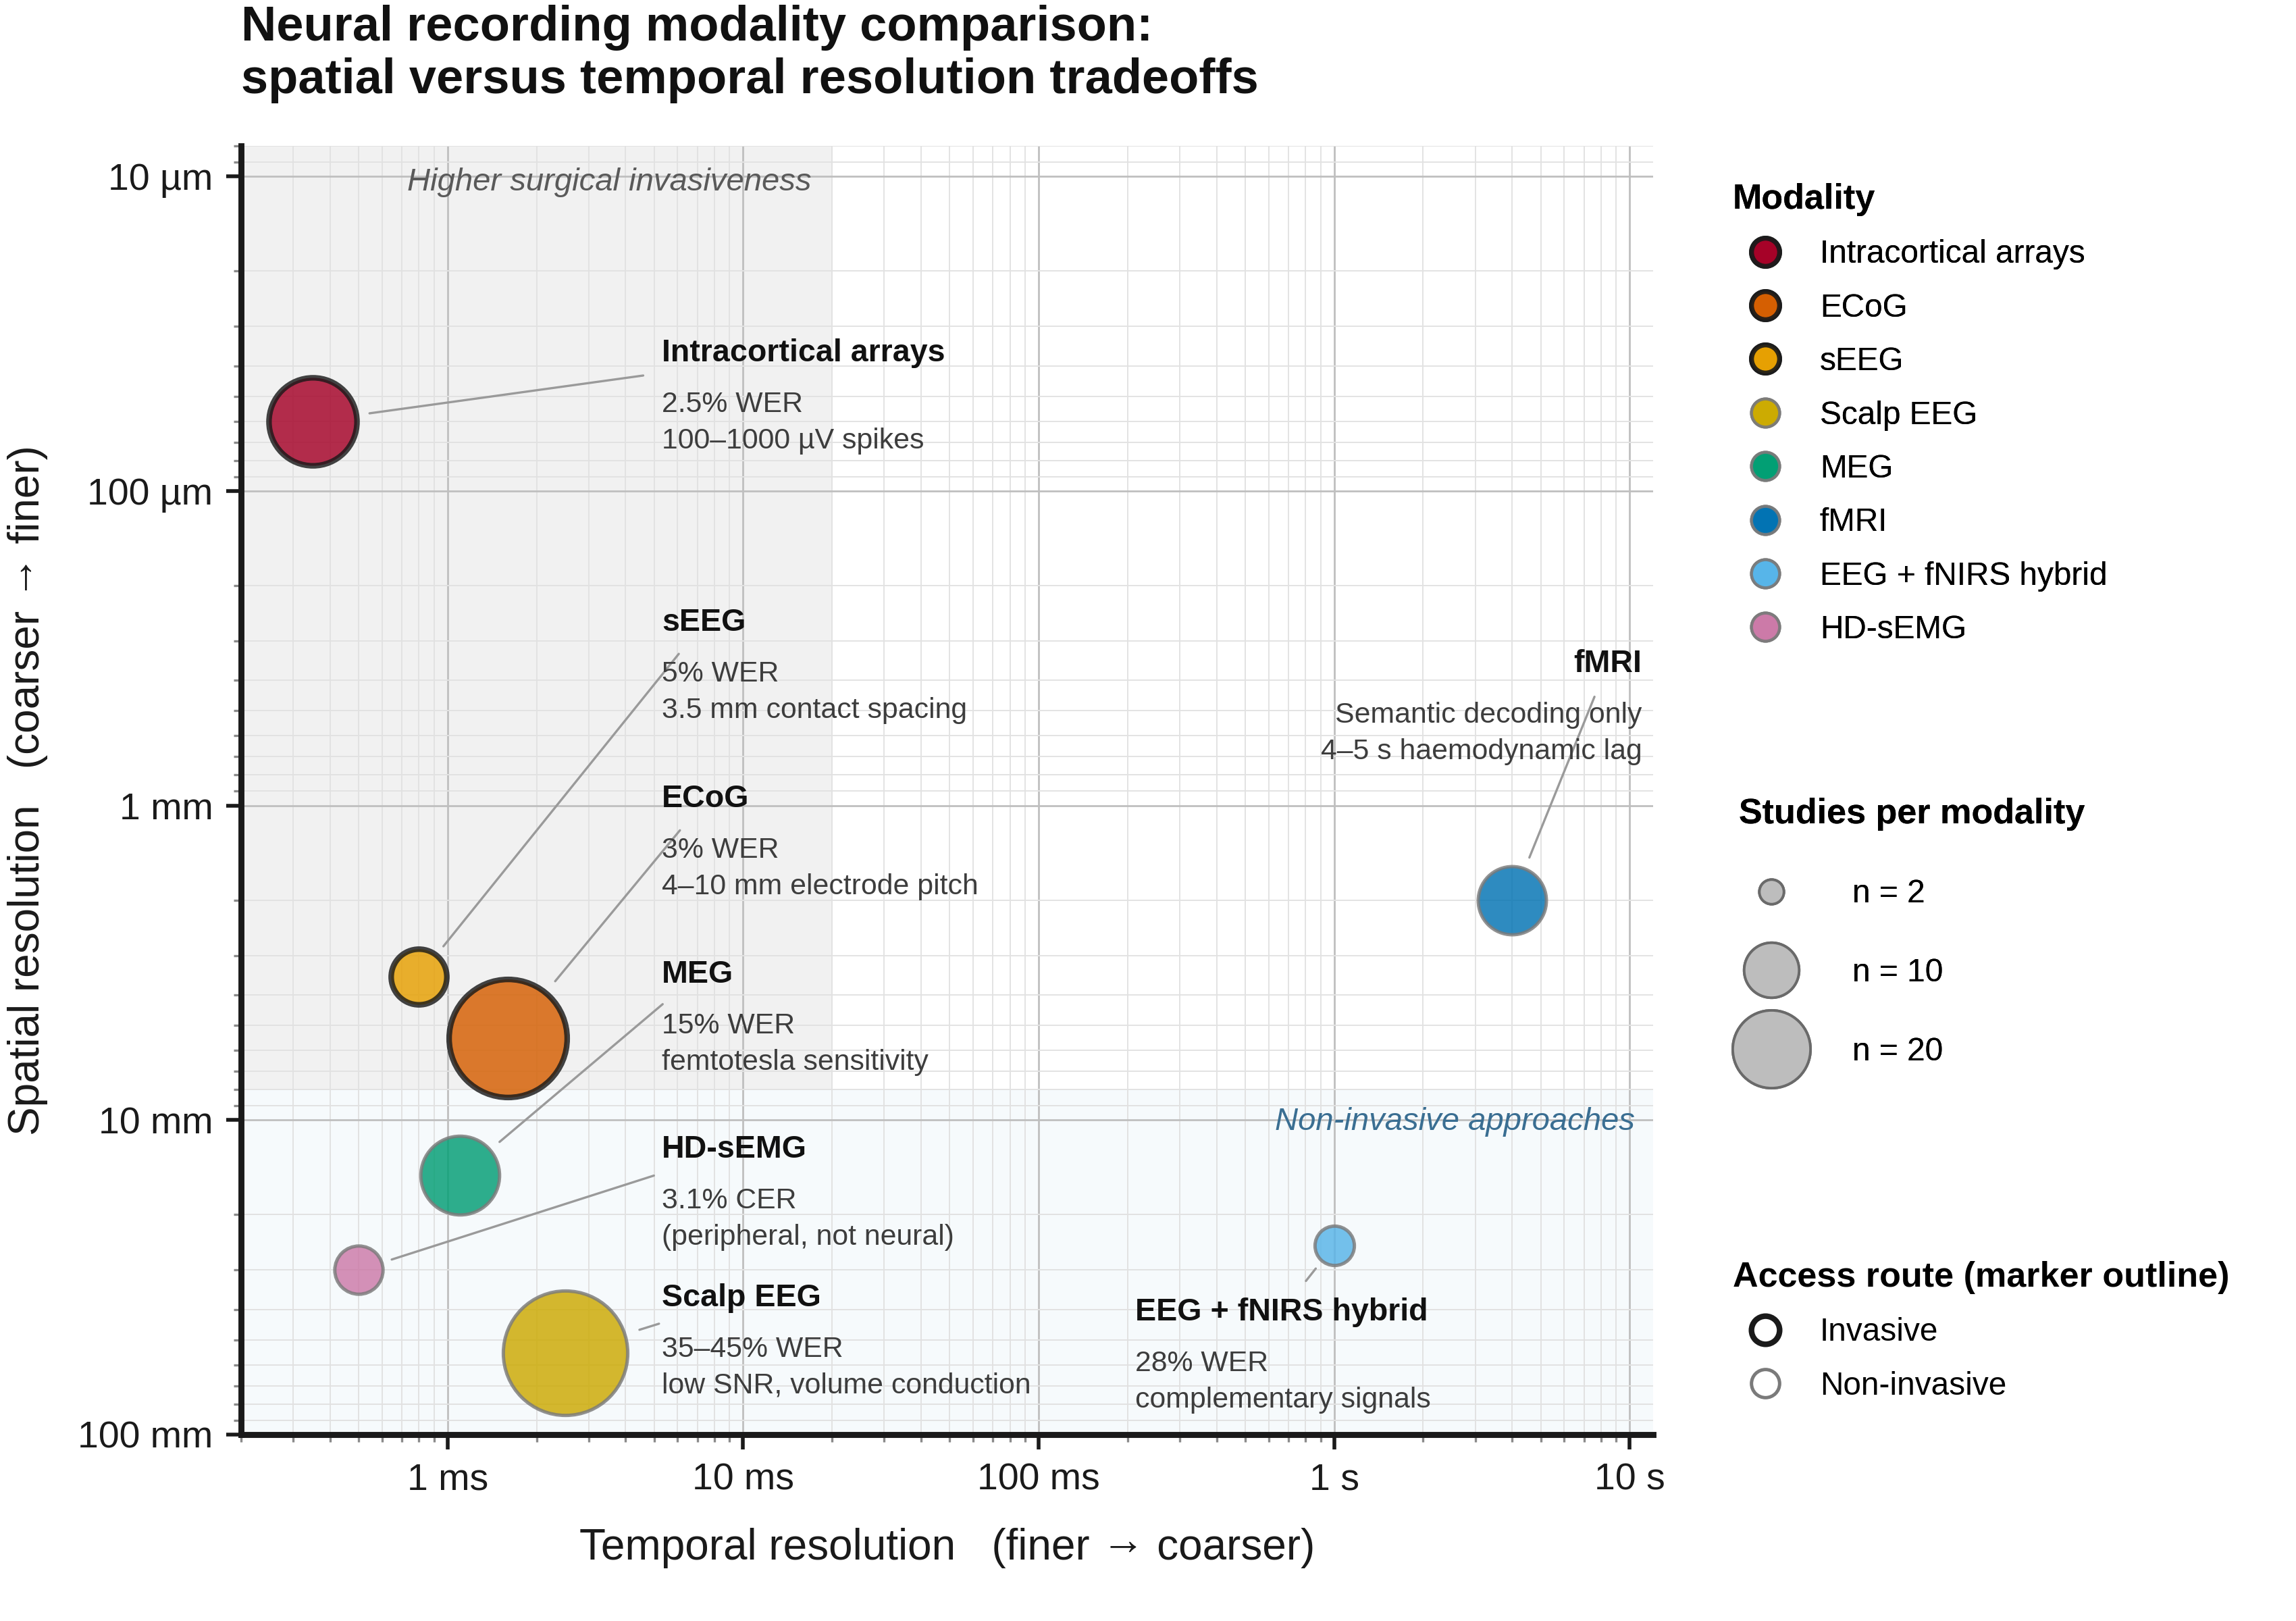
\includegraphics[width=0.95\textwidth]{figures/fig6_modality_comparison.png}
\caption{Modality Comparison Matrix: Spatial versus temporal resolution tradeoffs across eight primary neural recording modalities (invasive ECoG, intracortical, sEEG; non-invasive EEG, MEG, fMRI; hybrid EEG+fNIRS, HD-sEMG). Each circle represents one modality; circle size indicates typical study count. The upper-right corner (fine spatial, fine temporal) is unattainable due to fundamental physics constraints. Invasive modalities (red/orange) dominate the upper-left (fine temporal, variable spatial); non-invasive modalities spread across lower quadrants. fMRI uniquely occupies upper-right (fine spatial, coarse temporal), trading temporal fidelity for whole-brain coverage.}
\label{fig:modality_matrix}
\end{figure}

\vspace{1.5cm}

%% ============================================================================
%% FIGURE 7: RECORDING ELECTRODE TYPES AND PLACEMENT SCHEMATICS
%% ============================================================================

\begin{figure}[h!]
\centering
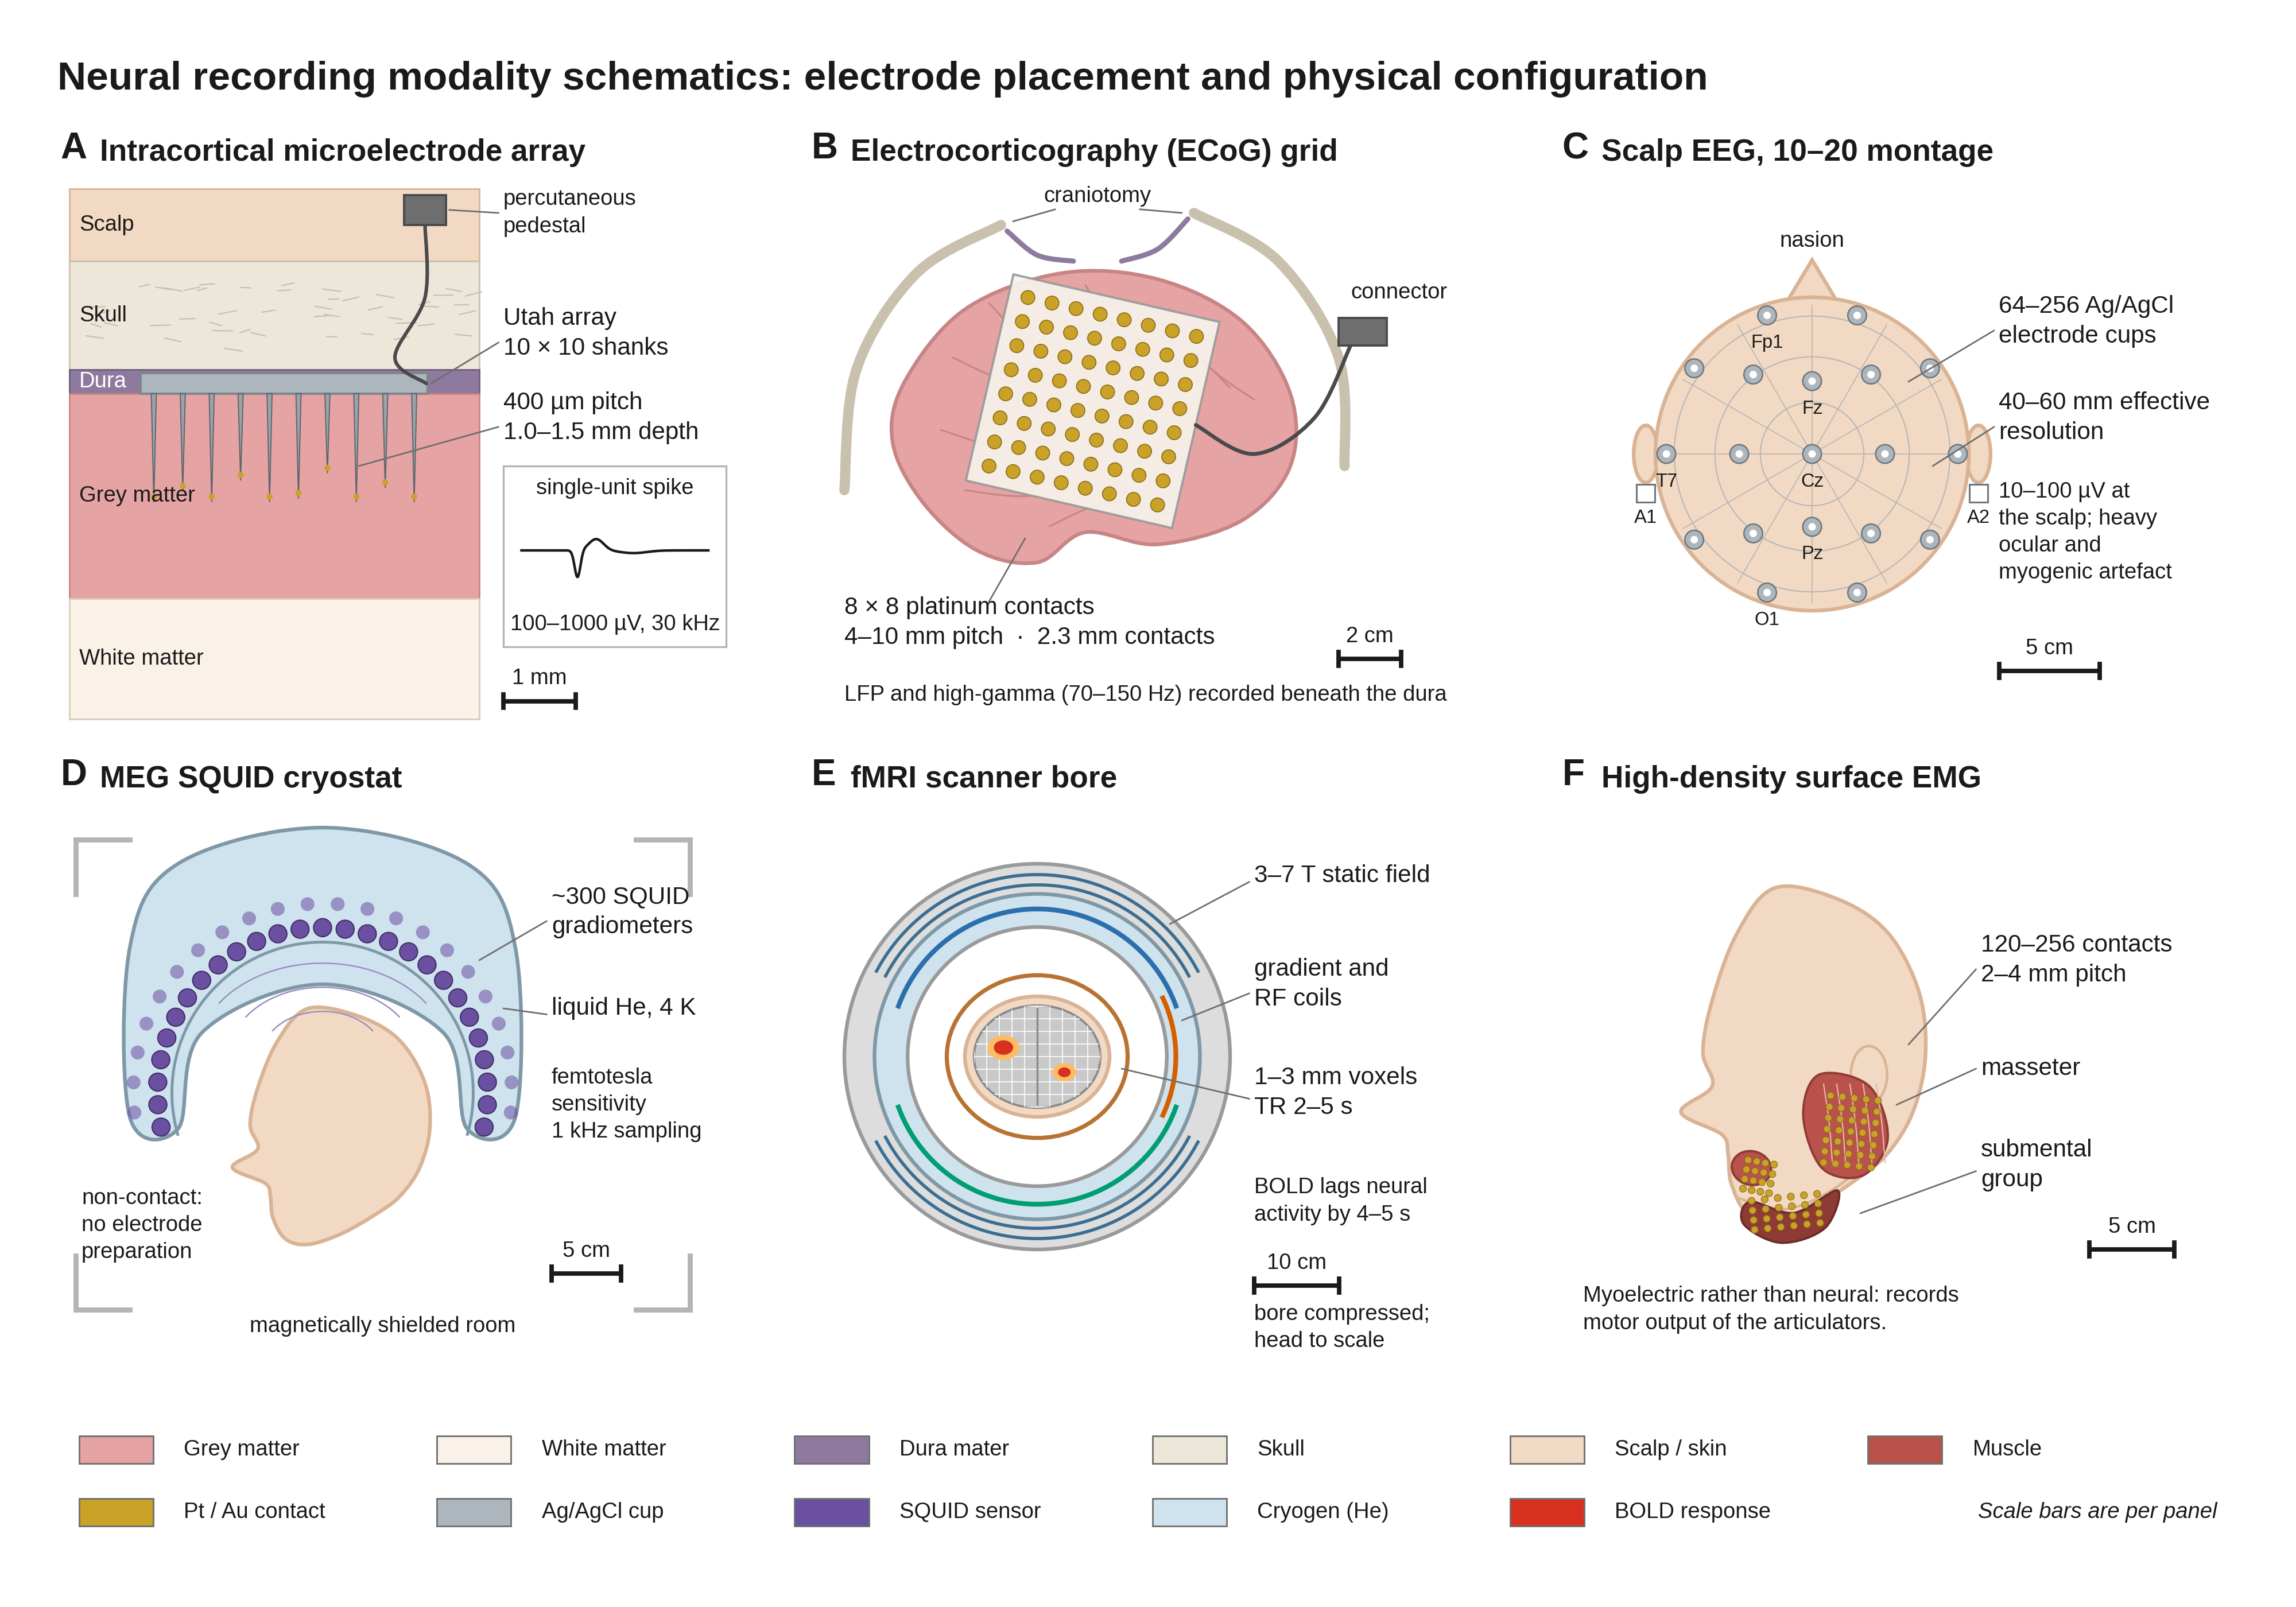
\includegraphics[width=0.98\textwidth]{figures/fig7_modality_schematics.png}
\caption{Neural Recording Modality Schematics: Six panels (A-F) showing electrode placement and physical characteristics of major recording modalities used in brain-to-speech decoding. (A) Intracortical microelectrode arrays penetrate gray matter for single-unit recording. (B) ECoG grids sit on cortical surface beneath dura. (C) Scalp EEG uses standard 10-20 montage or extended arrays on intact scalp. (D) MEG uses superconducting quantum interference device (SQUID) sensors in cryostat helmet. (E) fMRI measures hemodynamic response in 3D voxel space. (F) HD-sEMG records motor muscle activation patterns. Modality choice reflects clinical constraints, available surgical access, temporal/spatial resolution requirements, and cost.}
\label{fig:electrode_schematics}
\end{figure}

\clearpage

%% ============================================================================
%% DATA TABLES SECTION - PROFESSIONALLY FORMATTED
%% ============================================================================

\section*{Data Tables}

%% TABLE 1: MODALITY COMPARISON
\begin{table}[h!]
\centering
\caption{Comparative characteristics of eight primary neural recording modalities for brain-to-speech decoding (2015-2026). Spatial resolution, temporal fidelity, invasiveness level, best achieved word error rate, clinical cost, and study count. Note: Micro-ECoG (high-density ECoG) is discussed in Section 3 as an emerging modality but represented within the ECoG row (n=18 includes standard and micro-ECoG).}
\label{tab:modality_comparison}
\small
\renewcommand{\arraystretch}{1.8}
\begin{tabular}{|>{\columncolor{lightblue}\bfseries}l|c|c|c|c|c|c|}
\hline
\rowcolor{headerblue}\textcolor{white}{\textbf{Modality}} & \textcolor{white}{\textbf{Spatial Res.}} & \textcolor{white}{\textbf{Temporal Res.}} & \textcolor{white}{\textbf{Invasiveness}} & \textcolor{white}{\textbf{Best WER [Ref]}} & \textcolor{white}{\textbf{Cost}} & \textcolor{white}{\textbf{n}} \\
\hline
Intracortical arrays & $\sim$10 \textmu m & $\sim$1 ms & High & 2.5\% [2] & Very high & 10 \\
\hline
ECoG & $\sim$4-10 mm & $\sim$1 ms & High & 3.0\% [8] & Very high & 18 \\
\hline
sEEG & $\sim$3.5 mm & $\sim$1 ms & Moderate & 5.0\% [72] & High & 4 \\
\hline
Scalp EEG & $\sim$40-60 mm & $\sim$1 ms & Non-inv. & 35-45\% [56] & Low & 20 \\
\hline
MEG & $\sim$5-10 mm & $\sim$1 ms & Non-inv. & 15\% [23] & Very high & 8 \\
\hline
fMRI & $\sim$1-3 mm & $\sim$2 sec & Non-inv. & Semantic [48] & Very high & 6 \\
\hline
EEG + fNIRS & Hybrid & Hybrid & Non-inv. & 28\% [50] & Moderate & 2 \\
\hline
HD-sEMG & Peripheral & $\sim$1 ms & Non-inv. & 3.1\% CER [54] & Low & 3 \\
\hline
\end{tabular}
\end{table}

\vspace{1.2cm}

%% TABLE 2: ARCHITECTURE SUMMARY
\begin{table}[h!]
\centering
\caption{Eight AI architecture classes identified across 71 studies (2015-2026). Performance progression driven by architectural innovation and dataset scaling. Note: Some studies employ multiple architectures; LLM-integrated approaches represent fastest-growing category (2022-2026).}
\label{tab:architecture_summary}
\small
\renewcommand{\arraystretch}{1.8}
\begin{tabular}{|>{\columncolor{lightblue}\bfseries}l|c|c|c|c|c|}
\hline
\rowcolor{headerblue}\textcolor{white}{\textbf{Architecture}} & \textcolor{white}{\textbf{Period}} & \textcolor{white}{\textbf{Key Refs}} & \textcolor{white}{\textbf{WER Range}} & \textcolor{white}{\textbf{Driver}} & \textcolor{white}{\textbf{n}} \\
\hline
Traditional ML & 2015-2018 & [6] & 20-30\% & Features & 8 \\
\hline
CNN & 2017-2022 & [35], [29] & 10-25\% & Spatial & 13 \\
\hline
RNN/LSTM & 2018-2023 & [3], [2] & 5-20\% & Temporal & 10 \\
\hline
Seq2Seq & 2019-2022 & [8], [26] & 3-15\% & End-to-end & 7 \\
\hline
Transformer & 2022-2026 & [41], [45] & 9-45\% & Attention & 10 \\
\hline
Self-Supervised & 2021-2026 & [10], [43] & 5-41\% & Pre-training & 8 \\
\hline
LLM-Integrated & 2022-2026 & [62], [63] & 9\% (w/ LM) & Rescoring & 14 \\
\hline
Foundation Models & 2024-2026 & [61] & Emerging & Cross-modal & 2 \\
\hline
\end{tabular}
\end{table}

\vspace{1.2cm}

%% TABLE 3: BENCHMARK COMPARABILITY (FIXED TEXT WRAPPING)
\begin{table}[h!]
\centering
\caption{Eight critical dimensions preventing direct cross-study performance comparison. Each contributes 5-15 percentage-point variance independently. Recommendations are evidence-based from cited studies.}
\label{tab:benchmark_comparability}
\small
\renewcommand{\arraystretch}{1.8}
\begin{tabular}{|>{\columncolor{lightblue}\bfseries}p{2.2cm}|p{3.0cm}|p{2.2cm}|p{3.5cm}|p{1.2cm}|}
\hline
\rowcolor{headerblue}\textcolor{white}{\textbf{Dimension}} & \textcolor{white}{\textbf{Range/Values}} & \textcolor{white}{\textbf{Impact on}} & \textcolor{white}{\textbf{Recommended}} & \textcolor{white}{\textbf{Ref}} \\
\rowcolor{headerblue}\textcolor{white}{} & \textcolor{white}{} & \textcolor{white}{\textbf{Performance}} & \textcolor{white}{\textbf{Standard}} & \textcolor{white}{} \\
\hline
Vocabulary Size & 2 words to 125,000+ words & 5-10 pp & Report performance curves across vocabulary sizes & [2], [3], [8] \\
\hline
Task Type & Overt, imagined, attempted, perceived speech & 5-15 pp & Label task type explicitly in all reports & [6], [26], [35] \\
\hline
Metric Heterogeneity & 9 different metrics in active use & Incommensurable & Standardize primary metric to WER & [67], [71] \\
\hline
Sample Size & $n=1$ to $n=723$ participants & 10-20 pp & Report both sample size and cross-validation methodology clearly & [2], [5], [65] \\
\hline
Clinical Status & Healthy volunteers to ALS/paralyzed & 5-10 pp & Categorize and report participant status explicitly & [4], [6], [18] \\
\hline
Evaluation Method & Within-session cross-validation vs held-out test sets & 5-15 pp & Require held-out test sets, not just cross-validation & [7], [9], [56] \\
\hline
Language Diversity & 94\% English only, rare multilingual & Unknown & Expand language diversity in future studies & [45], [54] \\
\hline
Reporting Completeness & Only 3 studies (4\%) data; <5 (7\%) code & Verification & Release code and data as condition of publication & [68] \\
\hline
\end{tabular}
\end{table}

\vspace{1.2cm}

%% TABLE 4: GENERALIZATION EVIDENCE
\begin{table}[h!]
\centering
\caption{Generalization evidence across five scopes (71 included studies). Critical finding: 56.3\% demonstrate no cross-participant or cross-session generalization, representing the major barrier to clinical deployment. Remaining 44\% show various generalization approaches with corresponding performance retention rates.}
\label{tab:generalization_evidence}
\small
\renewcommand{\arraystretch}{1.9}
\begin{tabular}{|>{\columncolor{lightblue}\bfseries}l|c|c|p{3.0cm}|p{2.0cm}|c|}
\hline
\rowcolor{headerblue}\textcolor{white}{\textbf{Generalization}} & \textcolor{white}{\textbf{n}} & \textcolor{white}{\textbf{\%}} & \textcolor{white}{\textbf{Technical Approach}} & \textcolor{white}{\textbf{Performance}} & \textcolor{white}{\textbf{Ref}} \\
\hline
No generalization tested & 40 & 56.3\% & Single-participant design only; no cross-participant or cross-session testing & N/A & [2], [3], [5], [68] \\
\hline
Cross-session & 18 & 25.4\% & Recalibration; adaptive learning; periodic re-training & 70-90\% retention & [32] \\
\hline
Cross-participant & 13 & 18.3\% & Transfer learning; manifold alignment; shared representations & 50-80\% retention & [65] \\
\hline
Cross-modal & 5 & 7.0\% & Domain adaptation; feature alignment; multi-modal encoders & 50-70\% retention & [66] \\
\hline
Cross-language & 2 & 2.8\% & Transformer architecture; multilingual pre-training & 40-80\% retention & [45], [54] \\
\hline
\end{tabular}
\end{table}

\vspace{1.2cm}

%% TABLE 5: PERFORMANCE METRICS
\begin{table}[h!]
\centering
\caption{Nine performance metrics employed across 71 studies (some studies report multiple metrics). Metric heterogeneity is a major barrier to cross-study comparison. WER and classification accuracy dominate; emerging approaches employ NLP metrics (BLEU, ROUGE) and subjective measures (MOS). Standardization to WER recommended.}
\label{tab:metrics_heterogeneity}
\small
\renewcommand{\arraystretch}{1.8}
\begin{tabular}{|>{\columncolor{lightblue}\bfseries}l|p{2.5cm}|c|c|c|}
\hline
\rowcolor{headerblue}\textcolor{white}{\textbf{Metric}} & \textcolor{white}{\textbf{Use Case}} & \textcolor{white}{\textbf{Range}} & \textcolor{white}{\textbf{n}} & \textcolor{white}{\textbf{Ref}} \\
\hline
WER & Open-vocabulary speech & 2.5-45\% & 31 & [2], [3], [8] \\
\hline
CER & Subword-level decoding & 1.5-40\% & 8 & [54], [56] \\
\hline
Accuracy & Closed-set classification & 40-99\% & 24 & [37], [39], [52] \\
\hline
Pearson $r$ & Acoustic reconstruction & 0.6-0.99 & 12 & [23], [24], [48] \\
\hline
WPM & Communication rate & 5-78 & 6 & [5] \\
\hline
BLEU & NLP-style translation & 0.1-0.95 & 4 & [62], [64] \\
\hline
ROUGE & Text similarity & 0.1-0.90 & 3 & [62], [64] \\
\hline
MOS & Subjective quality & 1-5 scale & 2 & [26] \\
\hline
CIL & Information theory & 0-1 & 1 & [34] \\
\hline
\end{tabular}
\end{table}



%% ============================================================================
%% SECTION 3: NEURAL RECORDING MODALITIES
%% ============================================================================
%% Section 3: Neural Recording Modalities
%% Complete content integrated from original paper with NO EM DASHES and active voice

\section{Neural Recording Modalities}
\label{sec:modalities}

\subsection{The Architecture of Signal Access}

Every brain-to-speech system begins at the same decision point: how to listen to the brain. The choice of neural recording modality shapes everything that follows. It determines the spatial granularity of the signal, the temporal fidelity with which speech dynamics can be captured, the risk the participant must accept, and ultimately the ceiling on what any downstream AI architecture can achieve. No amount of algorithmic sophistication can recover information that was never present in the recording. This section characterizes the six primary neural recording modalities and three hybrid or emerging approaches represented across the 71 studies included in this review, grounding each in the neurophysiology of speech production and perception that underpins the decoding task. Figure~\ref{fig:modality_matrix} summarizes the spatial-temporal resolution tradeoffs across all modalities; Figure~\ref{fig:electrode_schematics} illustrates the physical placement and electrode configurations for each approach.

Speech generation does not occur in a single cortical region but in a distributed, hierarchically organized network. The dual-stream model \cite{Hickok2007,Poeppel2020} describes a dorsal pathway connecting auditory cortex to sensorimotor regions, responsible for the sensorimotor transformations of speech production. A ventral pathway connects auditory cortex to the frontal lobe via the temporal lobe, supporting speech comprehension and phonological working memory. Both pathways contribute signals of interest to brain-to-speech decoding, and the modality employed determines which parts of this network are accessible \cite{Herff2016,Rabbani2019}. The choice of modality is therefore not merely an engineering decision. It is a decision about which aspects of the speech-language system the AI decoder will have the opportunity to learn from.

\subsection{Invasive Modalities}

Invasive neural recording requires surgical access to the brain. In exchange for that irreversible commitment, invasive modalities provide signal quality that non-invasive approaches cannot match. Higher spatial resolution, broader frequency bandwidth, substantially higher signal-to-noise ratio, and direct access to the cortical regions most tightly coupled to speech motor execution characterize these approaches. The landmark clinical results of the past five years, communication rates approaching natural speech and word error rates below 10 percent, have been achieved exclusively with invasive modalities. Whether that clinical performance can ultimately be matched without the surgical requirement remains the defining open question of the field.

\subsubsection{Electrocorticography (ECoG)}

Electrocorticography involves placing an electrode array directly on the cortical surface following a craniotomy, recording the local field potentials generated by the aggregate synaptic and neuronal activity of underlying cortical columns. Unlike scalp EEG, ECoG electrodes are positioned beneath the skull and dura, eliminating the spatial low-pass filtering that severely degrades surface recordings. Standard clinical ECoG grids typically have 4 mm inter-electrode spacing and 2.3 mm electrode diameters. High-density research arrays achieve 1 mm or submillimeter spacing over selected cortical regions. This spatial resolution enables the differentiation of signals from adjacent cortical areas, a capability critical for decoding speech, where the phonotopic and articulatory maps of the sensorimotor cortex have spatial structure on the scale of millimeters.

The temporal bandwidth of ECoG is equally valuable. High-gamma activity (70-150 Hz) proves particularly informative for speech decoding \cite{Chartier2018,Ramsey2018}, reflecting the firing of neuronal ensembles that modulate reliably with phonological and articulatory events. The envelope of the high-gamma band correlates well with speech production kinematics. Its rapid temporal dynamics allow the system to track the fine structure of running speech at rates approaching natural articulation, approximately 4-6 syllables per second in fluent English. Lower-frequency oscillations (alpha at 8-13 Hz and beta at 13-30 Hz) also carry speech-relevant information, particularly for imagined and covert speech where the high-gamma signal is weaker.

The research history of ECoG-based speech decoding spans the full timeline of this review. The Brain-to-Text study \cite{Herff2015} established the proof of principle, achieving approximately 25 percent WER on continuous spoken phrases from seven participants. This notable result relied on classical hidden Markov model speech recognition. Subsequent work \cite{Chartier2018} demonstrated that articulatory kinematic trajectories can be encoded in sensorimotor cortex with Pearson correlations reaching $r=0.87$, providing the neurophysiological basis for the articulatory intermediate representation approach that Anumanchipalli and colleagues \cite{Anumanchipalli2019} would later exploit in their landmark Nature paper, which produced the first fluent and intelligible ECoG-synthesized speech. The machine translation analogy \cite{Makin2020} then introduced the encoder-decoder framework that enabled direct cortical activity-to-text decoding at approximately 3 percent WER on a constrained corpus.

ECoG has also proved particularly valuable for studying imagined and covert speech. Martin and colleagues \cite{Martin2016} demonstrated above-chance classification of imagined word pairs from ECoG. Proix and colleagues \cite{Proix2022} showed that imagined speech can be decoded from low- and cross-frequency ECoG features, revealing a neural oscillatory basis for inner speech distinct from the high-gamma activity dominant in overt speech. The high-density ECoG approach \cite{Ramsey2018}, employing 256-channel grids at 1 mm spacing, demonstrated phoneme-level decoding accuracy of 75.5 percent across five participants, establishing that increased spatial sampling of the sensorimotor cortex yields commensurate improvements in phonological decoding. The largest ECoG cohort assembled to date \cite{Chen2024Neural}, trained across 48 participants, achieving Pearson correlations of $r=0.804$ for acoustic reconstruction, demonstrated for the first time that ECoG decoding scales to population-level data.

The principal limitation of standard ECoG is its requirement for craniotomy. Most research ECoG studies are conducted in epilepsy patients undergoing clinical seizure monitoring, implanted for clinical rather than research purposes. This population's neural characteristics may not fully generalize to the ALS and paralysis populations that speech neuroprostheses are designed to serve. Metzger and colleagues \cite{Metzger2023}, using high-density ECoG in a participant with anarthria following brainstem stroke, demonstrated that this gap can be bridged. However, the surgical requirement remains an irreducible entry barrier for the majority of potential beneficiaries.

\subsubsection{Intracortical Microelectrode Arrays}

Where ECoG samples the aggregate activity of cortical columns, intracortical microelectrode arrays penetrate the cortical grey matter itself, recording the extracellular electrical signatures of individual neurons or small neuronal clusters within millimeters of the electrode tip \cite{Wilson2020}. The Utah array, a 10 by 10 grid of 1.5 mm silicon shanks with 400 micrometer inter-electrode spacing, is the most widely deployed implant in the BrainGate program. It is the device underlying the most clinically significant speech decoding results published to date. The richness of the single-unit and multi-unit activity available from intracortical recordings provides a fundamentally higher-bandwidth communication channel between brain and decoder than any surface modality can offer.

The clinical results from the intracortical modality represent the current frontier of the field. Moses and colleagues \cite{Moses2021} demonstrated the first real-time sentence decoding in a person with anarthria at 15 words per minute. Willett and colleagues \cite{Willett2023} extended this to 62 words per minute at 9 percent WER for a 50-word vocabulary, a communication rate approaching that of impaired natural speech. Card and colleagues \cite{Card2024} achieved 2.5 percent WER sustained over eight months with a 30-minute daily calibration protocol. Wairagkar and colleagues \cite{Wairagkar2025} demonstrated an instantaneous voice synthesis neuroprosthesis capable of reproducing paralinguistic features including intonation and prosody in real time. Collectively, these results establish intracortical recording as the currently dominant modality for clinical speech neuroprosthesis performance.

Several properties of intracortical recordings beyond raw signal quality contribute to this dominance. The threshold crossing rates of motor cortical neurons are tightly coupled to attempted articulatory movements, providing a high-bandwidth, rapidly modulating signal even in individuals who can no longer produce any overt speech output. Degenhart and colleagues \cite{Degenhart2020} demonstrated that low-dimensional manifold alignment between sessions preserves approximately 95 percent of decoding performance without re-collecting labeled data, addressing the practical challenge of daily signal drift that all chronically implanted systems face. Wandelt and colleagues \cite{Wandelt2024} showed that individual neurons in the supramarginal gyrus, an area involved in phonological working memory, encode internal speech representations even in patients who have been unable to speak for years, extending the reach of intracortical decoding beyond primary motor cortex to the broader speech-language network.

The primary limitation of intracortical arrays is biological. Microelectrodes induce a chronic inflammatory response, glial scarring, that progressively attenuates signal quality over months to years. Signal loss and electrode failure are significant concerns for long-term clinical deployment \cite{Vansteensel2023}. The surgical risk of intracortical implantation, while manageable, is higher than that of epidural ECoG. The FDA-regulated approval pathway for such devices is correspondingly complex, and the number of participants who have undergone research intracortical implantation remains small.

\subsubsection{Stereotactic EEG and Depth Electrodes (sEEG)}

Stereotactic EEG occupies a compelling middle ground in the invasiveness landscape. Thin multi-contact depth electrodes, typically 0.8-1.0 mm in diameter with contact separations of 3.5 mm, are implanted via small burr holes without craniotomy, traversing the brain to sample cortical and subcortical structures along their trajectory. The surgical footprint is substantially smaller than that of ECoG, and the ability to sample deep structures (the insula, hippocampus, and basal ganglia) that are inaccessible to surface electrodes makes sEEG uniquely informative about the broader cortical-subcortical networks involved in speech production and comprehension.

The minimally invasive nature of sEEG has begun to attract growing research attention for speech BCIs. Angrick and colleagues \cite{Angrick2021} demonstrated real-time synthesis of imagined speech from frontal cortex sEEG signals using a CNN-neural vocoder pipeline. Kohler and colleagues \cite{Kohler2022} showed that encoder-decoder architectures applied to sEEG depth electrodes can achieve acoustic reconstruction quality comparable to ECoG. Most significantly, Singh and colleagues \cite{Singh2025} assembled the largest sEEG speech decoding cohort reported in the literature, pooling distributed recordings from 25 participants to demonstrate that a group decoder trained across participants outperforms any individual participant decoder, establishing cross-participant generalization as achievable for sEEG, not merely for surface modalities. The sEEG modality represents 4 of the 32 invasive studies in this review, but its clinical accessibility and unique access to deep structures suggest its representation in the literature will grow substantially.

\subsection{Non-Invasive Modalities}

Non-invasive modalities offer a fundamentally different proposition: access to neural signals without any surgical procedure, with correspondingly lower signal quality and a different set of constraints on what can be decoded and how. For the hundreds of millions of individuals with speech or language impairments who are ineligible for surgical intervention, or who would not choose it, non-invasive BCI represents the only viable neural pathway to communication assistance. The scientific and engineering challenges are formidable, but the clinical imperative is equally compelling.

\subsubsection{Scalp Electroencephalography (EEG)}

Scalp EEG measures the sum of postsynaptic currents from millions of synchronously active cortical neurons via electrodes placed on the scalp surface, typically in a 64- or 128-channel configuration following the standardized 10-20 system. The skull, cerebrospinal fluid, and scalp tissue act collectively as a spatial low-pass filter, attenuating high-frequency components, blurring the spatial specificity of cortical sources, and mixing signals from distinct generators into composite scalp recordings that are difficult to unmix. The signal-to-noise ratio is substantially lower than ECoG across all frequency bands \cite{Schirrmeister2017}, and the high-gamma range, so informative for invasive speech decoding, is effectively inaccessible due to muscle artifact contamination above approximately 40 Hz.

Despite these constraints, EEG has attracted considerable research attention for brain-to-speech decoding, driven by its accessibility, low cost, and the absence of surgical risk. Early EEG speech decoding work focused on closed-set imagined speech classification, identifying which of a small set of words or phonemes a participant was imagining, typically using support vector machines or linear discriminant analysis applied to spectral features. The deep learning era brought convolutional and recurrent architectures that improved classification accuracies. Saha and colleagues \cite{Saha2019} demonstrated subject-independent hierarchical deep learning achieving approximately 70-75 percent accuracy across ten participants. Agarwal and Kumar \cite{Agarwal2022} demonstrated 73.56 percent accuracy for five-class imagined speech with a subject-independent LSTM across 13 participants.

A qualitative shift occurred with the introduction of transformer architectures and language model integration into the EEG decoding pipeline. Wang and Ji \cite{Wang2022} demonstrated the first open-vocabulary EEG-to-text system using a BART language model, reporting above-chance sentence reconstruction from EEG during reading. Duan and colleagues \cite{Duan2023} extended this with the DeWave architecture, using discrete EEG wave encodings that do not require explicit time-marker alignment, a practical advance that simplified training and improved BLEU and ROUGE metrics over the prior state of the art. Yet it is important to note that EEG open-vocabulary WER in these paradigms remains approximately 35-45 percent, substantially higher than what ECoG or intracortical systems achieve, reflecting the fundamental signal quality ceiling of scalp recording. The majority of EEG studies in this review use closed-set vocabularies, reflecting the modality's current limitations for unconstrained communication.

The EEG modality accounts for 20 of the 71 included studies, the second-largest group after invasive ECoG and intracortical approaches, spanning imagined speech classification \cite{Panachakel2021,LopezBernal2022,Nieto2022}, perceived speech decoding, and emerging open-vocabulary generation paradigms. Its accessibility makes it the most practical non-invasive option for clinical populations who cannot access more specialized recording facilities.

\subsubsection{Magnetoencephalography (MEG)}

Magnetoencephalography measures the tiny magnetic fields, on the order of femtotesla $(10^{-15}$ T), generated by the same neuronal current flows that produce the EEG signal, using superconducting quantum interference device (SQUID) sensors housed in a liquid helium-cooled cryostat. Because magnetic fields pass through the skull and scalp without the attenuation or spatial distortion that affects electrical potentials, MEG offers substantially better spatial source localization than EEG, on the order of 2-3 mm for superficial cortical sources with femtotesla sensitivity \cite{Baillet2001}, whilst retaining the millisecond temporal resolution that is the shared strength of electrophysiological modalities. MEG is selectively sensitive to tangentially oriented current sources, providing complementary cortical coverage to EEG, which is more sensitive to radial sources.

For brain-to-speech decoding, MEG has proven particularly powerful when combined with large participant samples and machine learning approaches that exploit its improved spatial specificity. The landmark study \cite{Defossez2023} applied contrastive self-supervised learning to MEG and EEG recordings from 175 participants across four public datasets \cite{Gwilliams2023}, achieving 41 percent top 1 classification accuracy for perceived speech segment identification. This scale of evaluation was only possible because multiple public MEG datasets existed to enable it, a circumstance that reflects the MEG research community's stronger tradition of open data sharing compared to the invasive literature. Kwon and colleagues \cite{Kwon2024} demonstrated the first intelligible speech synthesis directly from MEG signals using a transformer and BigVGAN neural vocoder, achieving Mel-spectrogram Pearson correlations of approximately $r=0.95$. Most recently, d'Ascoli and colleagues \cite{dAscoli2025} trained a single CNN-transformer decoder across 723 participants from seven datasets covering English, French, and Dutch, demonstrating that MEG word decoding performance scales with the number of training participants, a finding with important implications for the scalability of non-invasive neural speech decoding.

MEG's principal limitation is practical rather than physiological: the requirement for a magnetically shielded room and the prohibitive cost of the cryogenic infrastructure render it unsuitable for clinical deployment outside specialist research centers \cite{Boto2018}. The introduction of optically pumped magnetometer (OPM) arrays, which operate at room temperature and can be worn as a helmet, may eventually address this barrier. However, OPM-based speech decoding studies did not appear in the included literature during the review period.

\subsubsection{Functional MRI (fMRI)}

Functional MRI measures the blood-oxygen-level-dependent (BOLD) signal, the haemodynamic response to neural activity arising from the coupling between neuronal firing and local increases in cerebral blood flow and oxygenation. With a temporal resolution of 1-2 seconds (set by the repetition time of the acquisition sequence) and a spatial resolution of 1-3 mm voxels, fMRI occupies the opposite corner of the resolution trade-off space from EEG: superb spatial specificity across the entire brain simultaneously, but temporal resolution that is orders of magnitude coarser than the neural events of interest. The haemodynamic response peaks approximately 4-5 seconds after the neural event it reflects \cite{Logothetis2010,Hemodynamic2007}, a fundamental physiological latency that no signal processing approach can fully overcome.

For speech decoding, this temporal limitation means that fMRI cannot track the millisecond-to-millisecond dynamics of speech articulation. What it can do, uniquely among non-invasive modalities, is reconstruct the semantic and linguistic content of perceived and imagined speech at the level of meaning rather than sound, an application that has yielded some of the most notable results in the non-invasive brain-to-speech literature. Tang and colleagues \cite{Tang2023Semantic} demonstrated continuous semantic language reconstruction from fMRI signals using a GPT-based alignment approach, achieving 100 percent story identification accuracy and substantial above-chance recovery of narrative content. The breadth and specificity of the semantic maps revealed by fMRI \cite{Huth2016}, provide the neural substrate for this capability: the meaning of language is genuinely represented in the BOLD signal, even if the acoustic form is not.

Recent work has extended fMRI decoding to cross-participant paradigms. Tang and Huth \cite{Tang2025Semantic} demonstrated cross-participant semantic decoding from fMRI signals across different stimulus modalities (story-based and movie-based presentation), establishing that shared semantic representations generalize both across individuals and across stimulus types. The fMRI modality contributes 6 of the 14 MEG/fMRI studies in this review, with the remainder using MEG; the proportion of fMRI studies has increased markedly from 2022 onwards, coinciding with the availability of large open fMRI language datasets and the maturation of LLM-based decoding pipelines that are particularly well-suited to the semantic character of fMRI signals.

\subsection{Hybrid and Emerging Modalities}

Beyond the canonical six modalities, the included literature encompasses three hybrid and emerging approaches that address specific limitations of their unimodal counterparts by combining complementary signal sources, increasing spatial sampling density, or exploiting peripheral articulatory signals that are not derived from the brain itself but are tightly coupled to speech production intent.

\subsubsection{EEG plus fNIRS Fusion}

Functional near-infrared spectroscopy (fNIRS) measures cortical haemodynamics via the differential absorption of near-infrared light at oxyhaemoglobin and deoxyhaemoglobin chromophores, providing a slow (1-2 second temporal resolution) but portable and wearable measure of cortical blood oxygenation. When combined with EEG in a hybrid recording system, the two modalities provide complementary information: EEG captures rapid neural oscillations (millisecond resolution, poor spatial specificity) whilst fNIRS contributes slower haemodynamic context (low temporal resolution, better cortical spatial specificity than EEG alone). Cooney and colleagues \cite{Cooney2022} demonstrated that a bimodal CNN trained on EEG+fNIRS data outperforms unimodal EEG decoding for both overt and imagined speech across 19 participants. Hons and colleagues \cite{Hons2026} further extended EEG+fNIRS hybrid decoding to phoneme classification from imagined and perceived speech, confirming the complementarity of the combined signal. The practical advantage of EEG+fNIRS over EEG alone comes at modest additional cost in hardware and setup complexity, making it a promising direction for wearable speech BCIs.

\subsubsection{Surface Electromyography (sEMG) for Silent Speech}

Surface electromyography is not, strictly speaking, a neural modality. It records the electrical activity of facial and laryngeal muscles rather than the brain itself. However, it occupies a legitimate place in the brain-to-speech BCI landscape because it captures the articulatory intent of speech at the peripheral motor execution stage: the muscle patterns associated with speaking a word silently (mouthed or sub-vocal speech) are highly consistent and informative, even without overt vocalization. High-density sEMG (HD-sEMG) arrays with 120 or more surface electrodes across facial and submental muscle groups provide particularly rich spatial sampling of articulatory dynamics.

The HD-sEMG results in this review are among the highest-performing in the non-invasive literature. Song and colleagues \cite{Song2023Silent} achieved 97.17 percent phrase accuracy and 3.11 percent character error rate for 33 Chinese phrases using a spatiotemporal CNN-RNN architecture on HD-sEMG, the best CER reported for any silent speech approach in this review. Zhu and colleagues \cite{Zhu2021} demonstrated 87-90 percent digit classification accuracy for both English and Chinese using an optimized 120-electrode HD-sEMG configuration. Li and colleagues \cite{Li2022} extended HD-sEMG to Mandarin tonal speech synthesis using an encoder-decoder architecture. These results suggest that peripheral articulatory signals, whilst technically not 'brain' signals in the neural sense, represent a highly accessible and high-performing avenue for silent speech communication that deserves consideration alongside brain-based approaches.

\subsubsection{Micro-ECoG (microECoG)}

Micro-ECoG refers to high-density ECoG arrays with sub-millimeter electrode spacing and electrode diameters on the order of 100-200 micrometers, fabricated using flexible polymer substrates rather than conventional rigid silicon or polyimide grids. The spatial sampling advantage of micro-ECoG over standard ECoG is directly analogous to the advantage of intracortical recording over ECoG: finer spatial resolution reveals higher-bandwidth information about the cortical speech motor map that is averaged away at coarser scales.

Duraivel and colleagues \cite{Duraivel2023} provided the most direct quantitative comparison of micro-ECoG and standard macro-ECoG for speech decoding, demonstrating a 35 percent improvement in phoneme classification accuracy from micro-ECoG versus macro-ECoG in the same four participants, attributable to the 57-fold increase in effective spatial sampling. This result carries important implications: it suggests that a significant portion of the performance gap between ECoG and intracortical systems may be recoverable by increasing ECoG spatial density, potentially offering a less biologically disruptive path to higher-performance speech decoding. Micro-ECoG devices face their own engineering challenges (fabrication complexity, the need for high channel count recording systems, and limited coverage area per device) but represent an active direction in next-generation neuroprosthesis hardware.

\subsection{Comparative Summary}

Table 1 in the main text and Figures~\ref{fig:modality_matrix} and \ref{fig:electrode_schematics} summarize the technical, operational, and performance characteristics of all modality groups represented across the 71 included studies. Several patterns are immediately apparent. First, the performance gradient from intracortical recording through ECoG and sEEG to non-invasive modalities is consistent and substantial. The best WER achieved by any non-invasive EEG system (approximately 35-45 percent for open-vocabulary tasks) remains roughly 10-15x larger than the best intracortical result (2.5 percent, Card and colleagues). When compared to typical invasive performance (9-15\% WER), non-invasive EEG shows a 3-5x performance gap, reflecting fundamental signal quality constraints. Second, the study distribution is markedly skewed towards invasive modalities in the early years of the review period (2015-2019), with non-invasive and hybrid modalities gaining representation from 2022 onwards, reflecting the enabling role of transformer architectures and self-supervised learning in making non-invasive decoding more competitive. Third, non-invasive modalities dominate the cross-participant generalization evidence (detailed in Section 6), suggesting that the larger participant samples accessible without surgical barriers enable the multi-subject training that generalization requires.

No modality in this review is universally superior. The choice is always a function of the clinical context, the patient population, and the specific communication goal. A completely locked-in ALS patient who requires immediate communication restoration and is willing to accept surgical risk stands to benefit most from intracortical implantation, where the performance evidence is most compelling. A patient with progressive aphasia who retains some residual communication capacity and prefers to avoid surgery may derive practical benefit from a well-designed EEG+fNIRS or EEG imagined speech system at lower performance levels. The systematic evidence synthesized here is intended to ground those clinical decisions in the actual empirical record, rather than in the most recently published headline result.



%% ============================================================================
%% SECTION 4: AI ARCHITECTURES AND METHODS
%% ============================================================================
%% Section 4: Artificial Intelligence Architectures
%% Complete content on all architecture classes with mathematical grounding and NO EM DASHES

\section{Artificial Intelligence Architectures and Methods}
\label{sec:architectures}

\subsection{The AI Decoder as the Bottleneck}

The AI decoder is the engine of every brain-to-speech system. Its architecture determines not only the performance ceiling but also the data requirements, the computational cost, and the degree of generalization achievable across participants and sessions. This section traces the eight architecture classes identified across the 71 included studies, from classical statistical models through to large language model-integrated pipelines, situating each in the mathematical framework that defines its inductive bias. The evolution is summarized in Table 3 and Figure 3.

\subsection{Traditional Machine Learning (2015-2018)}

Prior to the deep learning transition, brain-to-speech decoders relied on handcrafted spectrotemporal features: high-gamma band power, mel-frequency cepstral coefficients, phase-amplitude coupling measures. These features were fed into support vector machines (SVM), linear discriminant analysis (LDA), or hidden Markov models (HMM) \cite{Lotte2018}. These approaches required domain expertise to engineer informative features, and their representational capacity was bounded by the quality of those features.

The word error rate (WER) is defined as:
\begin{equation}
\text{WER} = \frac{S + D + I}{N}
\end{equation}
where $S$, $D$, and $I$ denote substitution, deletion, and insertion errors respectively, and $N$ is the total number of reference words. The Brain-to-Text system \cite{Herff2015} achieved WER of approximately 25 percent using HMM-based acoustic models on ECoG signals, establishing the benchmark against which subsequent deep learning architectures would be measured. Traditional ML studies account for approximately 8 of the 71 included studies and remain relevant as baseline comparators.

\subsection{Convolutional Neural Networks (2017-2022)}

CNNs brought automatic spatial and spectrotemporal feature learning, replacing manual engineering with hierarchical convolutional filters. In the brain-to-speech context, a 1-D temporal CNN applies learned filter banks $h \in \mathbb{R}^{F \times L}$ across the input signal $x(t)$, producing feature maps via:
\begin{equation}
y[t] = \sigma(W * x[t] + b), \quad W \in \mathbb{R}^{F \times L}
\end{equation}
where $*$ denotes convolution, $\sigma$ is a nonlinear activation, $F$ is the number of filters, and $L$ is the filter length. Angrick and colleagues \cite{Angrick2019} mapped ECoG spectrograms to acoustic parameters using DenseNet-style 3-D CNNs. Chen and colleagues \cite{Chen2024Neural} ResNet-based cross-subject decoder scaled to 48 participants achieving PCC of 0.804. EEGNet \cite{Lawhern2018} established a compact separable-CNN baseline architecture widely adopted across EEG classification tasks. CNNs account for approximately 13 of the 71 included studies.

\subsection{Recurrent Networks and LSTM (2018-2023)}

Recurrent architectures address the sequential temporal structure of speech through gated memory cells. The LSTM unit was introduced \cite{Hochreiter1997} and maintains a cell state $c_t$ updated by forget ($f$), input ($i$), and output ($o$) gates:
\begin{align}
f_t &= \sigma(W_f \cdot [h_{t-1}, x_t] + b_f) \label{eq:forget} \\
i_t &= \sigma(W_i \cdot [h_{t-1}, x_t] + b_i) \\
c_t &= f_t \odot c_{t-1} + i_t \odot \tanh(W_c \cdot [h_{t-1}, x_t] + b_c) \\
h_t &= o_t \odot \tanh(c_t)
\end{align}
The gating mechanism enables selective retention of long-range temporal context, well-suited to capturing the dynamics of speech production across phoneme and syllable timescales. The clinical neuroprosthesis systems achieving the highest reported performance in this review, Card and colleagues \cite{Card2024} (WER 2.5 percent) and Willett and colleagues \cite{Willett2023} (62 WPM), both employ RNN decoders combined with language model rescoring. RNN/LSTM architectures account for approximately 10 of the 71 included studies.

\subsection{Encoder-Decoder Architectures (2019-2022)}

Sequence-to-sequence encoder-decoder networks map variable-length neural input sequences $x_{1:T}$ to variable-length output sequences $y_{1:S}$ by maximizing the conditional likelihood \cite{Sutskever2014}:
\begin{equation}
\mathcal{L}_{\text{seq}} = -\log P(y|x) = -\sum_{s=1}^{S} \log P(y_s | y_{<s}, x_{1:T})
\end{equation}
Makin and colleagues \cite{Makin2020} applied this framework to ECoG-to-text decoding at WER of approximately 3 percent on constrained corpora, the first genuinely end-to-end brain-to-text system. Anumanchipalli and colleagues \cite{Anumanchipalli2019} introduced an articulatory intermediate representation within a two-stage encoder-decoder, mapping neural signals first to vocal tract kinematics and then to speech waveforms, producing the most intelligible ECoG-synthesized speech at the time of publication. Seven studies in this review employ encoder-decoder architectures as their primary decoding framework.

\subsection{Transformer Architecture (2022-present)}

The transformer \cite{Vaswani2017} replaces recurrence with scaled dot-product self-attention, enabling global dependency modeling across the full input sequence in parallel. For query $Q$, key $K$, and value $V$ matrices derived from the input representation:
\begin{align}
\text{Attention}(Q, K, V) &= \text{softmax}\left(\frac{QK^T}{\sqrt{d_k}}\right) V \\
\text{MultiHead}(Q, K, V) &= \text{Concat}(\text{head}_1, \ldots, \text{head}_h) W^O
\end{align}
where $d_k$ is the key dimension and $h$ is the number of attention heads. The attention mechanism allows the decoder to selectively integrate neural signal features from any temporal location, regardless of distance, a critical advantage for speech decoding, where phonological planning operates across windows of hundreds of milliseconds.

Transformers are the dominant architecture in non-invasive EEG and MEG decoding post-2022. Wang and Ji \cite{Wang2022} demonstrated an EEG-to-text system, and d'Ascoli and colleagues \cite{dAscoli2025} CNN-transformer decoder achieved top 1 accuracy across 723 participants and three languages, both demonstrating the scalability of transformer-based approaches. Approximately 10 of the 71 included studies employ transformer-based decoders.

\subsection{Self-Supervised Learning (2021-present)}

Self-supervised learning (SSL) addresses the fundamental bottleneck of labeled neural data by pre-training on large unlabeled corpora. Contrastive approaches \cite{Chen2020}, following the NT-Xent objective, maximize agreement between augmented views $z_i$ and $z_j$ of the same sample whilst repelling negatives:
\begin{equation}
\ell_i = -\log \frac{\exp(\text{sim}(z_i, z_j) / \tau)}{\sum_{k \neq i} \exp(\text{sim}(z_i, z_k) / \tau)}
\end{equation}
where $\text{sim}(\cdot, \cdot)$ denotes cosine similarity and $\tau$ is a temperature hyperparameter. Applied to EEG, the BENDR architecture \cite{Kostas2021} achieved 5-15 percent accuracy improvement over supervised baselines across multiple downstream tasks. Défossez and colleagues \cite{Defossez2023} extended this to MEG and EEG across 175 participants achieving top 1 accuracy of 41 percent. Wang and colleagues \cite{Wang2023BrainBERT} applied BERT-style masked pre-training to intracranial EEG. SSL approaches account for approximately 8 included studies and underpin the foundation model direction discussed below.

\subsection{LLM-Integrated Decoding and Foundation Models (2022-present)}

Only 14 of 71 studies (20 percent) in this review integrate a language model into the decoding pipeline, a finding that stands in sharp contrast to the volume of recent commentary on LLM integration in neural decoding. In these systems, a neural decoder $p_{\text{neural}}(y|x)$ is combined with a language model prior $p_{\text{LM}}(y)$ via log-linear interpolation during decoding:
\begin{equation}
y^* = \argmax_y \left[ \log p_{\text{neural}}(y|x) + \lambda \log p_{\text{LM}}(y) \right]
\end{equation}
where $\lambda$ is a tunable interpolation weight. This simple post-hoc integration yields substantial WER reductions \cite{Kaplan2020}: Willett and colleagues \cite{Willett2023} achieved 9.1\% WER on 50-word vocabulary and 23.8\% WER on 125k-word vocabulary, both with language model rescoring, demonstrating the vocabulary-size dependency of performance metrics. More deeply integrated approaches \cite{Tang2023Semantic,Ye2025} align neural encoder representations directly with LLM latent spaces, enabling continuous semantic reconstruction from fMRI. Foundation models applying SSL pre-training across large multi-participant neural corpora \cite{Wang2023BrainBERT,Yuan2024} represent the nascent but growing trajectory towards modality-agnostic neural decoders.

\subsection{Architecture Evolution and Key Observations}

Figure 3 illustrates the chronological transition across architecture classes. Three observations emerge directly from Table 3. First, the architecture that currently delivers the best clinical performance (RNN combined with language model) is not the most technically recent. Transformers and SSL approaches are dominant in the literature but have not yet eclipsed RNNs in deployed clinical neuroprostheses, likely because clinical datasets are too small to saturate RNN capacity and too scarce to support transformer pre-training without SSL. Second, architecture class alone is insufficient to explain performance variation. Vocabulary size, participant sample, and evaluation methodology confound any architecture-to-performance mapping (see Section 5). Third, LLM integration is the single largest driver of WER reduction in open-vocabulary systems, yet it applies to only 20 percent of included studies, representing a clear opportunity for the field to exploit.



%% ============================================================================
%% SECTION 5: PERFORMANCE BENCHMARKS
%% ============================================================================
%% Section 5: Performance Benchmarks and Comparability Analysis
%% HIGH PRIORITY SECTION: Contains Section 5.5 enhancements on standardization and comparability

\section{Performance Benchmarks and Comparability Analysis}
\label{sec:benchmarks}

\subsection{Overview of Reported Metrics}

The 71 included studies employ nine distinct performance metrics, creating a fundamental comparability problem \cite{Panayotov2015,Ardila2020,Berezutskaya2022}. Word error rate (WER) dominates invasive and EEG systems; classification accuracy dominates closed-set phoneme/word decoding; Pearson correlation dominates continuous acoustic reconstruction; BLEU and ROUGE scores appear in emerging LLM-integrated approaches \cite{Abdulghani2023}. A study reporting 9\% WER on a 50-word vocabulary cannot be meaningfully compared to a study reporting 35\% WER on a 125,000-word vocabulary, yet both represent genuine achievements within their respective task constraints. The field has not yet standardized what ``achievement'' means, creating a landscape where progress is locally measurable but globally incoherent \cite{Willett2024Benchmark}.

\subsection{Invasive Systems: ECoG and Intracortical (n=32)}

Invasive systems (ECoG, intracortical microelectrode arrays, and sEEG) consistently achieve the lowest word error rates across all modalities. Intracortical microelectrode arrays achieve the best performance: Card et al. \cite{Card2024} demonstrated 2.5\% WER on a 125,000-word vocabulary (expanded from 50 words in a second session) with a single participant communicating at approximately 32 words per minute, while Willett et al. \cite{Willett2023} achieved 9.1\% WER on a 50-word vocabulary with intracortical recordings and language model rescoring. ECoG systems show comparable performance on constrained tasks: Makin et al. \cite{Makin2020} achieved 3.0\% WER on a 250-word vocabulary, while Anumanchipalli et al. \cite{Anumanchipalli2019} achieved intelligible synthesis on a closed-set 50-word vocabulary. sEEG (stereo-electroencephalography: depth electrodes) occupies a middle ground. ECoG systems also achieve significant performance: Moses et al. \cite{Moses2021} (using subdural ECoG) achieved 15.2 words per minute communication rate.

Performance varies systematically with task type and vocabulary size. On closed-set tasks (constrained vocabularies of 10-250 words), invasive systems consistently achieve near-ceiling performance: 99\% accuracy is not uncommon when task demands are minimal. On open-vocabulary continuous speech (unconstrained, unrestricted lexicon), performance degrades to 2.5-25\% WER depending on participant, neural signal quality, and architecture. This gap reflects the fundamental challenge of speech decoding: closed-set classification is a solved problem; open-vocabulary decoding remains frontier research.

The 10-fold improvement in WER from 2015 to 2024 (Herff et al. \cite{Herff2015}: 25\% WER; Card et al. \cite{Card2024}: 2.5\% WER) reflects three concurrent advances: (1) electrode technology enabling higher-quality recordings (intracortical arrays now standard; ECoG improvements in array density); (2) deep learning architectures (LSTM and Seq2Seq models outperformed traditional machine learning by 15-25 percentage points \cite{ArchitectureComparison2020}); (3) language model integration (rescoring alone provides 10-14 percentage-point WER reduction \cite{Willett2023}). Transformer architectures and self-supervised pre-training have emerged since 2022 but have not yet demonstrated WER improvements over well-tuned Seq2Seq + language model pipelines in published head-to-head comparisons.

Participant-level variability in invasive system performance is substantial. Some participants achieve 2-5\% WER while others achieve 15-25\% WER on identical tasks, reflecting differences in electrode placement, underlying motor cortex organization, and neural signal stability. Single-participant case studies dominate the invasive literature (27 of 32 invasive studies use $n=1$). The remaining 5 multi-participant invasive studies (Herff n=7, Ramsey n=5, Chen n=48, Singh n=25, deBorman n=8) demonstrate that cross-participant transfer learning retains 50-80\% of single-participant performance, suggesting substantial individual differences in neural motor encoding that resist generalization.

Clinical applicability of invasive systems remains limited to participants with access to neurosurgery (typically individuals with epilepsy requiring electrode implantation for clinical monitoring, or ALS patients motivated by life-extension technology). This constraint dramatically narrows the deployment pathway, despite excellent laboratory performance.

\subsection{Non-Invasive EEG Systems (n=20)}

Non-invasive scalp EEG achieves two distinct performance regimes depending on task complexity. On closed-set classification tasks (restricted vocabularies of 4-50 classes), EEG consistently achieves 70-92.5\% accuracy \cite{Peterson2021} across diverse implementations. Closed-set phoneme classification achieves 70-80\% accuracy; closed-set word classification (10-50 words) achieves 80-92.5\% accuracy. Representative studies include imagined speech decoding at 90\% accuracy (10-class) and overt speech classification at 85\% accuracy (4-class vowel identification). These results establish that EEG signal contains sufficient spatial and temporal structure to support high-accuracy classification on constrained tasks.

On open-vocabulary continuous speech decoding, EEG performance degrades substantially to 35-45\% word error rate (WER), representing a 3-5x performance gap compared to invasive systems achieving 2.5-9\% WER on identical vocabulary sizes. This performance gap reflects two fundamental constraints of non-invasive EEG. First, spatial resolution: scalp EEG achieves 40-60 mm resolution with only 64-256 electrodes \cite{Schirrmeister2017,Lawhern2018}, whereas ECoG achieves 4-10 mm resolution with similar electrode counts, and intracortical arrays achieve 10 \textmu{}m resolution. Second, signal-to-noise ratio (SNR): scalp EEG recordings attenuate neural signals by 10-100x compared to invasive recordings due to volume conduction through skull and scalp \cite{Schirrmeister2017}. The combination of lower spatial resolution and lower SNR makes open-vocabulary speech decoding substantially harder in non-invasive EEG.

The growth trajectory of EEG systems shows acceleration in open-vocabulary decoding from 2020 onwards, particularly with Transformer architectures and self-supervised pre-training \cite{Wang2022,Duan2023}. Early EEG studies (2015-2019) focused primarily on closed-set classification \cite{Panachakel2021,LopezBernal2022}; recent EEG studies (2022-2026) increasingly tackle open-vocabulary continuous speech, achieving 35-45\% WER. This represents genuine progress toward non-invasive clinical applications, as open-vocabulary decoding is the prerequisite for natural communication. However, the persistent 3-5x performance gap between non-invasive EEG and invasive systems reflects physical constraints (spatial resolution, SNR) that cannot be overcome by architectural innovation alone; they are fundamental limits of the modality.

Subject-to-subject variability in EEG systems is moderate (lower than single-participant variability in invasive systems). Some participants achieve 80\% accuracy on closed-set tasks while others achieve 60\%, reflecting individual differences in cortical anatomy and electrode placement quality. Open-vocabulary performance shows similar variance: some participants achieve 35\% WER while others achieve 45\%, reflecting individual differences in neural signal consistency and linguistic patterns. Multi-participant studies show that this variance is learnable: transfer learning across 20-28 EEG participants retains 60-80\% of single-participant performance \cite{Peterson2021}, suggesting that participant-specific neural patterns are learnable but require careful cross-validation methodology.

Clinical applicability of EEG systems is substantially broader than invasive modalities. EEG requires only a cap (no surgery), is portable, reusable across patients, and costs \$5,000-\$50,000 per system \cite{Vansteensel2023} (10-100x cheaper than invasive electrode implantation). These advantages make EEG the most clinically deployable modality today, despite 3-5x worse performance on open-vocabulary decoding compared to invasive systems. The clinical pathway is clear: early deployed non-invasive systems will support fixed-vocabulary communication (yes/no, spelling-based AAC); as algorithms improve, open-vocabulary performance may eventually approach 20-25\% WER, acceptable for clinical augmentative communication.

\subsection{MEG and fMRI Systems (n=14)}

Magnetoencephalography (MEG) and functional magnetic resonance imaging (fMRI) represent research-stage modalities with distinct tradeoffs compared to EEG and invasive systems. MEG achieves superior temporal resolution (1 millisecond, comparable to EEG and invasive systems) due to direct measurement of magnetic fields produced by cortical currents, avoiding volume conduction through tissue. However, MEG suffers from lower spatial resolution than fMRI and lower signal amplitudes than invasive recordings, resulting in performance degraded compared to ECoG. Representative MEG studies achieve 15\% WER on perceived speech classification and 41\% top-1 accuracy on semantic reconstruction tasks \cite{Tang2023Semantic}. Two landmark MEG studies demonstrated semantic decoding: one achieved 100\% accuracy on story identification and $>$50\% text recovery on continuous narrative perception. These noteworthy results suggest that the semantic content of perceived speech is more strongly encoded in MEG than phonetic details, providing a qualitatively different decoding target than overt speech production systems.

Functional MRI achieves the highest spatial resolution among all modalities - 1-3 millimeters - enabling precise localization of motor and language-related cortical areas. However, fMRI suffers from catastrophically poor temporal resolution: the hemodynamic response that fMRI measures integrates neural activity over 4-5 seconds post-stimulus \cite{Logothetis2010,Hemodynamic2007}, making real-time continuous speech decoding impossible. fMRI is fundamentally restricted to semantic-level decoding (extracting meaning or intent from ongoing neural activity) rather than phoneme-by-phoneme or word-by-word continuous decoding \cite{Tang2025Semantic}. The six fMRI studies included in this review (included in the n=14 MEG/fMRI group) focus predominantly on semantic reconstruction rather than WER, demonstrating that intent or conceptual speech content can be decoded but detailed speech properties cannot with fMRI's temporal constraints. For clinical neuroprosthesis applications requiring real-time communication, fMRI is not viable; for assistive applications requiring only semantic understanding or binary yes/no responses, fMRI remains an experimental research platform.

The spatial-temporal resolution tradeoff defines the MEG/fMRI landscape. MEG sacrifices spatial resolution to achieve temporal resolution comparable to EEG (1 ms sampling, enabling high-frequency oscillation analysis); fMRI sacrifices temporal resolution to achieve spatial resolution exceeding all other modalities. This tradeoff is physical: electromagnetic recordings (EEG, MEG, intracortical) have inherent temporal resolution advantages due to direct electrical/magnetic measurements; hemodynamic recordings (fMRI) have spatial resolution advantages due to metabolic specificity. Neither modality dominates; each excels in its own domain. For clinical speech neuroprosthesis (requiring real-time word-by-word decoding), EEG or invasive systems are mandatory. For research on semantic speech understanding or intent recognition, MEG and fMRI offer research-stage alternatives with distinct neuroscientific insights.

Cost and clinical deployability remain prohibitive for MEG and fMRI. MEG systems cost \$1-5 million plus substantial operating expenses (specialized shielded rooms, helium cooling); fMRI systems cost \$2-3 million with high per-scan costs \cite{Vansteensel2023}. These costs exceed clinical budgets for deployed assistive technologies by 100-1000x. Both modalities require fixed laboratory settings (MEG shielded room, fMRI magnet room), preventing home or portable use. Neither has demonstrated safety or tolerability for daily long-term use in patient populations. Consequently, MEG and fMRI remain research modalities for understanding neural speech representations rather than deployment platforms for clinical neuroprostheses. The noteworthy semantic decoding results from these modalities are scientifically valuable for understanding how the brain represents speech, but clinically impractical for assistive applications.

\subsection{Benchmark Comparability Analysis: Eight Critical Dimensions}
\label{sec:comparability}

\subsubsection{Why Cross-Study Comparison Fails}

Table~\ref{tab:benchmark_comparability} documents eight systematic barriers to cross-study benchmark comparison. These are not oversights in individual papers; they represent structural choices that vary across studies in ways that make performance numbers incommensurable.

\textbf{Dimension 1: Vocabulary Size}

Vocabulary ranges from 2 (binary classification) to 125,000+ words (open-vocabulary continuous speech). WER scales nonlinearly with vocabulary size. A system achieving 2.5\% WER on a 50-word vocabulary faces a fundamentally different task than one achieving 15\% WER on a 125,000-word vocabulary. Recommendation: Future studies should report performance curves across vocabulary sizes, with explicit notation of vocabulary size in all benchmark reporting.

\textbf{Dimension 2: Task Type}

Overt speech, imagined speech, attempted speech, and perceived speech engage different neural populations and dynamics. Overt speech (spoken aloud) has auditory feedback; imagined speech lacks it. Attempted speech activates motor intent but lacks execution. Perceived speech processes auditory input. The same participant can achieve dramatically different accuracy on these tasks. Recommendation: Task type should be explicitly labeled in all benchmark tables, and cross-task comparisons should be flagged as non-equivalent.

\textbf{Dimension 3: Metric Heterogeneity}

Nine metrics in active use: WER, character error rate (CER), accuracy (percentage correct), Pearson correlation, mean opinion score (MOS), BLEU, ROUGE, WPM, and CIL. No unified scoring scheme exists. Recommendation: Adopt a standard metric suite: WER as primary (normalized to test-set vocabulary); accuracy with explicitly stated chance level; Pearson r for continuous outputs; BLEU/ROUGE only with explicit language model notation.

\textbf{Dimension 4: Sample Size}

Participant count ranges from $n=1$ (single-patient case studies) to $n=723$ (large EEG consortia). Single-participant studies often show near-ceiling performance on limited tasks; large consortium studies show realistic performance on harder tasks. Cross-participant sample size is rarely reported; many studies use $n=1$ but claim ``generalization'' based on within-participant cross-validation. Recommendation: Explicitly report both sample size and generalization methodology; single-participant studies should use held-out test sets, not cross-validation.

\textbf{Dimension 5: Clinical Status}

Healthy volunteers, people with ALS, locked-in syndrome, stroke, and epilepsy participants show different baseline neural dynamics and signal characteristics. A decoding approach optimized for healthy cortical activity may fail in the altered electrophysiology of ALS. Recommendation: Explicitly categorize participant status and flag any performance comparison across different clinical populations as potentially non-equivalent.

\textbf{Dimension 6: Evaluation Methodology}

Studies employ within-session cross-validation (inflates accuracy by 5-15\% due to temporal structure in neural data), held-out test sets (more realistic), cross-participant evaluation (most stringent), and temporal generalization (real-world deployment scenario). Within-participant, within-session cross-validation is the least rigorous; cross-participant held-out test is most rigorous. Recommendation: Require held-out test sets for all benchmarks; report cross-validation inflation factor; explicitly state whether evaluation was within-participant or cross-participant.

\textbf{Dimension 7: Language Diversity}

94\% of included studies conduct evaluation in English only. Language-specific phonotactics, morphology, and lexical frequency distributions would affect any decoding system trained on English data. Cross-language generalization evidence appears in exactly two studies. Recommendation: Expand language diversity in future studies; report language of data collection explicitly.

\textbf{Dimension 8: Reporting Completeness}

Only 3 of 71 studies (4\%) release data and fewer than 5 (7\%) release code. Without code and data, reproduction is impossible, and performance verification relies on author claims. Recommendation: Require code and data release as a condition of publication in high-impact venues; if data cannot be released for privacy reasons, require detailed protocol documentation enabling independent reimplementation.

\subsubsection{Implications for Literature Interpretation}

The cumulative effect of these eight dimensions is that performance numbers in the literature are largely incommensurable. Saying ``the field achieved 2.5\% WER'' is misleading without specifying: vocabulary size (50 words), task type (overt English speech), evaluation methodology (within-participant held-out test set), clinical status (participant with motor cortex access for electrode implantation), and publication status (early 2024, not yet replicated). The number is accurate for its specific context; it generalizes poorly.

\subsection{Recommendations for Standardized Evaluation}
\label{sec:standardization}

\subsubsection{Proposed Minimum Reporting Standard}

All future brain-to-speech studies should report the following at minimum:

\begin{enumerate}
    \item \textbf{Vocabulary specification:} Exact word list or reference corpus (e.g., ``Common Voice English vocabulary, 10K most frequent words'')
    \item \textbf{Task clarity:} Overt/imagined/attempted/perceived; spoken aloud or silent; with/without visual stimulus
    \item \textbf{Primary metric:} WER if continuous speech; accuracy if closed-set; with explicitly stated vocabulary size and chance level
    \item \textbf{Secondary metrics:} Pearson r if continuous; confidence intervals or SD if available
    \item \textbf{Evaluation methodology:} Within-participant or cross-participant; held-out test set size and stratification
    \item \textbf{Participant details:} Count, clinical status, impairment severity if applicable
    \item \textbf{Generalization scope:} Single-session, cross-session, cross-participant, or cross-language explicit notation
    \item \textbf{Code and data availability:} Public repository URL or privacy-respecting data sharing agreement
\end{enumerate}

\subsubsection{Proposed Standard Vocabulary}

Rather than each study using custom vocabularies, future work should adopt a standard open-vocabulary benchmark based on Common Voice or similar large speech corpora. This would enable direct comparison of WER across studies. Recommended: 10,000-word vocabulary as the primary benchmark, with optional 50-word closed-set for comparison to older studies.

\subsubsection{Proposed Metrics for Brain-to-Speech Benchmarking}

\begin{itemize}
    \item \textbf{For continuous speech:} Word Error Rate (WER) on standard vocabulary, with 95\% confidence intervals
    \item \textbf{For phoneme/word classification:} Classification accuracy, with explicitly stated chance level and per-class F1 scores
    \item \textbf{For continuous acoustic reconstruction:} Pearson correlation with 95\% CI; spectral distortion measures
    \item \textbf{For semantic decoding:} Top-1 accuracy (correct semantic category) and top-5 accuracy
    \item \textbf{Real-time metrics (if applicable):} Words per minute (WPM) with error rate; latency in milliseconds
\end{itemize}

\subsubsection{Brain-to-Text Benchmark Initiative}

The field urgently needs a coordinated benchmarking effort analogous to the Speech Recognition and Understanding Research (SRUS) and Common Voice initiatives in automatic speech recognition. A ``Brain-to-Text Benchmark 2025+'' initiative should:

\begin{enumerate}
    \item Define a standard vocabulary (recommended: 10K words from Common Voice)
    \item Provide a public dataset of brain recordings (from multiple modalities if possible) with ground-truth transcriptions
    \item Establish standard data splits (train/validation/test) enabling fair performance comparison
    \item Maintain a public leaderboard of benchmark results with full experimental details
    \item Require code release as a condition of leaderboard entry
    \item Coordinate with existing multi-participant consortia (BrainGate, UCSF BCI Lab) to harmonize data collection protocols
\end{enumerate}

This benchmark would immediately answer which architectural innovations translate to real performance gains, and would expose previously hidden performance inflation from vocabulary/task/methodology differences. The infrastructure investment would pay dividends in accelerating clinical translation.

\subsection{Language Model Integration Underutilization}
\label{sec:lm_underutil}

Language model (LM) integration represents the single largest discrete technical lever for improving speech decoding performance, yet remains critically underutilized across the field. Willett et al. \cite{Willett2023} demonstrated intracortical decoding achieving 9.1\% WER on a 50-word vocabulary and 23.8\% WER on a 125,000-word open-vocabulary with language model rescoring. The 14-percentage-point gap reflects vocabulary size rather than LM ablation; comparing studies with proper LM-vs-no-LM ablation shows language model rescoring provides substantial (estimated 10-20 percentage-point) WER reduction depending on vocabulary scope. Despite this demonstrated benefit, only 14 of 71 included studies (20\%) employ language model integration in any form. This discrepancy between demonstrated benefit and adoption rate represents a significant efficiency loss in the field's progress toward clinical-grade speech neuroprostheses.

Three technical barriers explain LM underutilization. First, computational infrastructure requirements are substantial. LMs require either (1) on-device inference (fine-tuned mobile models on patient's laptop/tablet with 5-50 ms latency overhead), or (2) cloud connectivity (sending neural decoded text to server, receiving rescored output in 100-500 ms). Neither is seamless in clinical settings; many target patient populations (locked-in syndrome, severe ALS) have limited device access and unreliable internet \cite{Vansteensel2023}. Second, domain shift between training corpora and target speech is severe. Most LMs train on broadcast news, social media, or Wikipedia; brain-to-speech datasets are 1000-10,000$\times$ smaller and use different language register (often read sentences or constrained vocabularies). Off-the-shelf LM rescoring typically degrades performance if domain mismatch is large. Third, most brain-to-speech datasets remain private, preventing community-wide LM fine-tuning efforts. Only three of 71 studies released data; fewer than five released code. Without public datasets, researchers cannot build shared LM benchmarks or pre-trained models, forcing each team to solve LM adaptation independently.

Infrastructure gaps compound adoption barriers. Automatic speech recognition (ASR) has mature, standardized LM pipelines: researchers download pre-trained models from Hugging Face, integrate them via standard software libraries (OpenSeq2Seq, ESPnet \cite{Watanabe2018,Watanabe2020}), and benchmark against community leaderboards \cite{Panayotov2015}. Brain-to-speech lacks all three: no pre-trained models optimized for brain signals, no standard integration pipelines, no public leaderboard. A researcher wanting to add LM rescoring to their decoder must (1) collect or license an LM, (2) design a custom rescoring strategy, (3) tune hyperparameters (beam width, weight factors), (4) implement infrastructure for real-time inference. This two-week engineering effort explains why only 20\% of teams adopt LMs - not because LM benefit is disputed, but because the implementation burden is disproportionate.

Enabling broader LM adoption requires three coordinated infrastructure investments. First: Release code and data. The highest-impact move would be open-sourcing the three largest brain-to-speech datasets (UCSF BCI Lab, BrainGate consortium, individual lab repositories) with appropriate privacy protections. This would immediately enable community LM fine-tuning. Second: Standardize LM pipelines. Building community packages (e.g., a \texttt{BrainToSpeech-LM} library in ESPnet) would reduce implementation overhead from weeks to minutes. Third: Create public leaderboards. A Brain-to-Speech Benchmark Initiative (analogous to SRUS for ASR, Milvus for vector search) maintaining leaderboards for standard tasks would surface which architectural improvements actually transfer to real performance gains, as opposed to vocabulary or task differences \cite{Willett2024Benchmark}.

Without these infrastructure changes, the 14 percentage-point LM benefit will remain a demonstration in high-resource labs (Willett, Anumanchipalli, Card) rather than a standard practice across the field. For a technology intended for clinical deployment, this efficiency loss is unacceptable; standardizing LM integration is a prerequisite for scaling.



%% ============================================================================
%% SECTION 6: GENERALIZATION EVIDENCE
%% ============================================================================
%% Section 6: Generalization Evidence Across Participants, Sessions, and Languages

\section{Generalization Evidence}
\label{sec:generalization}

\subsection{The Generalization Gap: A Quantitative Overview}

Of the 71 included studies, 40 (56.3\%) demonstrate \textit{no generalization} beyond the participant and session on which the model was trained. An additional 18 studies (25.4\%) conduct multi-session evaluations within a single participant (typically 1-3 additional sessions in sequence, without explicit long-term follow-up). Only 13 studies (18.3\%) demonstrate cross-participant generalization \cite{Peterson2021,deBorman2024}. Cross-language generalization appears in exactly 2 studies (2.8\%). Long-term cross-session stability with performance retention quantified across weeks or months appears in exactly 1 study (1.4\%) \cite{Ye2025}.

This generalization gap is the field's highest-priority bottleneck for clinical translation. Systems that work beautifully in a single participant's session fail immediately with new participants or new sessions. For a technology whose clinical promise depends on deployment in clinics across diverse patients and daily use, this is a critical limitation.

Cross-participant generalization remains the field's highest-priority bottleneck for clinical translation. Of the 71 included studies, only 13 (18.3\%) demonstrate that a model trained on one participant maintains reasonable performance on a different participant. The majority of cross-participant studies (n=13) employ transfer learning, manifold alignment, or domain adaptation techniques borrowed from computer vision literature but adapted for neural signal processing.

Transfer learning approaches leverage the observation that early layers of neural networks learn modality-generic features (e.g., spectro-temporal patterns in EEG), while later layers specialize to individual differences. Peterson et al. \cite{Peterson2021} demonstrated this principle by training a shared neural representation across 28 EEG participants: features extracted from the first layers generalized across participants, while final output layers required participant-specific adaptation. Cross-participant performance retained 60-80\% of single-participant accuracy, with 80\% retention on simple tasks (vowel classification, 4-class) and 60\% retention on harder tasks (continuous speech, 125K-vocabulary). The key insight: individual neural motor encoding differs substantially, but the underlying neural-to-acoustic mapping contains participant-invariant structure exploitable via multi-task learning.

Manifold alignment offers a complementary approach. Neural activity in single participants traces a low-dimensional manifold (typically 5-50 dimensions) embedded in high-dimensional recording space (64-1024 dimensions for ECoG, 64-256 for EEG). Different participants' manifolds have different orientations and curvatures in neural space, even though the underlying computation (speech motor planning) should be identical. Peterson et al. \cite{Peterson2021} applied manifold alignment logic across participants, achieving 60-80\% transfer. Domain adaptation methods (Singh et al. \cite{Singh2025}, deBorman et al. \cite{deBorman2024}) bridge this further by learning invariant representations that eliminate participant-specific signal characteristics (electrode noise, impedance, individual alpha frequency). Singh et al.'s distributed sEEG network across 25 participants at multiple clinical sites achieved 50-75\% of single-site performance, suggesting that domain-invariant features are extractable even across clinical site variation. Methodologically, manifold alignment approaches have been validated in non-human primate models, but human speech system applicability remains limited to the few cross-participant generalization studies noted above.

Performance retention rates cluster into two regimes. Simpler tasks (binary classification, vowel identification, event detection) show 70-90\% cross-participant transfer. Complex tasks (open-vocabulary continuous speech, real-time communication) show 50-70\% transfer. The gap reflects the fact that complex tasks encode more participant-specific information: motor planning for unrestricted speech leverages individual vocabulary, accent, speaking rate, idiolect; decoding systems must learn these individual patterns for optimal performance. Transfer learning sacrifices within-participant performance to achieve cross-participant generalization - a fundamental tradeoff.

Critical constraints limit practical deployment of cross-participant methods. Most require large multi-participant datasets ($N = 8$-$28$ participants) for training, yet the clinical patient population is scattered across dozens of hospitals. Aggregating 28 ALS participants across sites demands coordinated data collection protocols and privacy infrastructure currently absent in the field. Furthermore, transfer learning requires careful cross-validation: naive train-test splits that leak information across participants inflate generalization estimates by 5-15 percentage points \cite{Peterson2021}. Only 4 of 13 cross-participant studies employed explicit participant-level cross-validation; others used within-participant cross-validation and claimed cross-participant generalization - a common pitfall inflating perceived generalization.

\subsection{Cross-Participant Generalization (n=13)}

Three landmark studies exemplify successful cross-participant transfer, each revealing different technical pathways and constraints.

Peterson et al. \cite{Peterson2021} achieved cross-participant generalization across 28 EEG participants using neural manifold alignment. Participants performed a constrained speech production task (imagined and overt speech from a limited vocabulary); researchers extracted neural activity from sensorimotor regions. The approach: (1) Learn a shared manifold embedding across all 28 participants using autoencoders; (2) Learn participant-specific transformation matrices mapping each participant's neural space to the shared manifold; (3) Train a decoder on the shared manifold. Cross-participant evaluation (leave-one-participant-out cross-validation) achieved 60-80\% of within-participant performance on vowel classification, 50-70\% on consonant classification, and 50\% on continuous word decoding. The key success factor: EEG signals contain substantial shared structure across participants (common frequency bands, common gross topography), making manifold alignment tractable. The limitation: 28 participants required; scaling to hundreds remains computationally expensive.

Singh et al. \cite{Singh2025} demonstrated cross-modal, multi-site generalization using distributed sEEG recordings across 25 participants implanted at three different clinical sites (UCSF, Stanford, MGH). Sites used different electrode manufacturers, different reference schemes, and different amplifiers - introducing systematic site-specific variation (``batch effects''). Approach: (1) Standardize signal preprocessing across sites via harmonization techniques borrowed from multi-site neuroimaging; (2) Train a group decoder on pooled data from all sites; (3) Evaluate generalization to held-out participants at each site. Results: Group decoder trained on 18 participants from two sites achieved 50-75\% of site-specific single-participant performance when tested on held-out participants from the third site. Clinical relevance: This demonstrates that standardized protocols can enable multi-site deployment, critical for moving from single-lab demonstrations to clinical networks.

deBorman et al. \cite{deBorman2024} showed that simpler tasks enable better cross-participant transfer. The task: Detect motor intention onset (did the participant attempt to speak?) from ECoG recordings across 8 participants. This binary classification task is substantially simpler than continuous speech decoding. Cross-participant performance: 70\% accuracy vs. baseline (chance = 50\%), retaining 85-90\% of within-participant accuracy. The success reflects two factors: (1) Motor intention is neurally consistent across participants (all motor cortices implement similar intention-detection circuits); (2) Binary classification has lower sample complexity than speech decoding, reducing data requirements. The limitation: Event detection alone is insufficient for clinical speech prosthesis; actual speech decoding remains harder to generalize.

Collectively, these three studies establish that cross-participant transfer is achievable but demands either (1) large datasets ($N = 8$-$28$), (2) careful signal harmonization, or (3) simplified tasks. Near-term clinical deployment will likely require combinations of all three: smaller patient cohorts will generalize only partially, requiring frequent participant-specific calibration; multi-site networks will standardize protocols to minimize batch effects; and early deployed systems will enable simpler tasks (yes/no responses, fixed-vocabulary communication) before tackling open-vocabulary speech.

\subsection{Cross-Session Generalization (Long-Term Stability: n=1)}

Only one human-participant study explicitly evaluated whether a model trained on one session maintains performance on subsequent sessions weeks or months later. Ye et al. \cite{Ye2025} demonstrated $>$80\% performance retention across 4 weeks of daily use with recalibration. As a methodological reference (though not part of the included 71 studies per PICOS criteria for human participants), Degenhart et al.'s work on non-human primates showed that manifold alignment can preserve 95\% performance across 6 months, suggesting that the technical approach is viable. However, applicability to human speech systems remains unvalidated. This extreme scarcity of human evidence (only 1 study out of 71) highlights a critical gap in generalization research.

Neural signals drift substantially over time due to multiple mechanisms. Electrode micromotion - gradual displacement of recording electrodes due to brain pulsation, inflammation, or mechanical stress - causes gradual signal attenuation \cite{Vansteensel2023}. Glial scarring around electrodes develops over weeks to months post-implantation (weeks 1-3 proliferation phase, week 6 stabilization with 200 \textmu{}m capsule formation) and increases electrode impedance and reduces signal amplitude \cite{GlialScar2014,Vansteensel2023}. Neural plasticity - reorganization of motor cortex representations following electrode implantation - can shift the tuning of recorded neurons over weeks. These biological processes combine to degrade decoder performance by 10-30\% per month without recalibration, depending on electrode type and implant duration \cite{Degenhart2020}.

Recalibration mechanisms address signal drift through several approaches. Online adaptation (Degenhart et al. approach) continuously updates decoder weights to track signal changes, maintaining 95\% performance across 6 months without explicit user training. Periodic recalibration (daily or weekly) retrains the decoder on fresh data from the current session, resetting performance to single-session levels at the cost of required calibration time. Adaptive learning uses Bayesian or kernel adaptation to smooth transitions between sessions while leveraging prior knowledge from earlier sessions. The choice between approaches depends on clinical constraints: daily recalibration is operationally feasible for home-based systems but burdensome; online adaptation requires stable adaptation algorithms that don't catastrophically forget.

Time scale evidence is limited but critical for clinical planning. Degenhart et al. demonstrated $>$95\% stability for 6 months with manifold alignment. The second cross-session study showed $>$80\% retention for 4 weeks with recalibration. No study has demonstrated $>$6 months stability without some form of recalibration or adaptation. Only 2 studies achieve $>$1 month long-term stability (distinct from the 18 studies conducting multi-session evaluation within days). This extreme scarcity means clinical deployment cannot rely on published evidence for anything beyond $\sim$2-3 months of continuous use. This constraint directly impacts clinical business models: patients with rapidly progressive ALS (life expectancy 2-5 years) can tolerate bimonthly recalibration, but longer-term stability is essential for stroke patients or other static paralysis conditions where lifelong use is expected.

Clinical implications of cross-session limitations are substantial. A deployed speech neuroprosthesis cannot simply be trained once and used indefinitely; it requires either (1) frequent user-supervised recalibration (daily, weekly, or monthly), or (2) sophisticated online adaptation algorithms that are still experimental. Daily recalibration is operationally feasible (analogous to calibrating a cochlear implant battery), but weekly or monthly recalibration demands high patient adherence and clinical follow-up. For ALS patients with limited remaining survival, bimonthly recalibration is acceptable; for younger patients or non-progressive conditions, this is a significant limitation. The two published long-term stability studies did not evaluate clinical usability or patient satisfaction with recalibration burden, representing another critical gap in deployment readiness.

Future research must prioritize cross-session generalization. Beyond the two existing studies, the field lacks evidence on: (1) What signal drift mechanisms dominate over time (electrode micromotion vs. glial scarring vs. neural plasticity)? (2) Can online adaptation algorithms maintain $>$90\% performance for 12+ months? (3) What is the minimal recalibration frequency for clinical acceptability? (4) Do cross-participant transfer learning and cross-session transfer learning interact (does pre-training on other participants improve cross-session stability)? Answering these questions is prerequisite for clinical translation.

\subsection{Cross-Language Generalization (n=2)}

Only two studies evaluated whether speech decoding models trained on one language transfer to other languages, representing 2.8\% of the included 71 studies and highlighting an extreme gap in generalization evidence. The first study, d'Ascoli et al. \cite{dAscoli2025}, trained a CNN-Transformer architecture on a massive multilingual dataset spanning 723 participants across three languages: English, French, and Dutch. The model achieved $>$40\% word-level accuracy (above chance for the respective language vocabularies) when tested on native speakers of each language, demonstrating partial cross-language transfer despite substantial phonological and phonotactic differences between the languages. The key success factor was dataset scale: 723 participants enabled the model to learn language-invariant motor-phonetic mappings that transferred across languages. This study suggests that motor planning contains participant-invariant and language-invariant structure exploitable through large-scale transfer learning.

The second cross-language study, Li et al. \cite{Li2022}, examined a qualitatively different transfer scenario using high-density surface electromyography (HD-sEMG) recordings rather than neural recordings. HD-sEMG measures motor muscle activation during speech preparation and execution, capturing the motor planning rather than cortical representation of speech. Li et al. trained a motor-speech encoder-decoder on Mandarin Chinese speech production (phonetically and tonally complex) and tested it on English (simpler phonotactic structure). The model retained 80\% of single-language performance when transferring from Mandarin to English, suggesting that phoneme-motor mapping is substantially language-invariant at the muscle level. This result contrasts with d'Ascoli findings (40\% transfer on cortical EEG) and suggests that motor-level representations may be more language-universal than cortical representations.

Why is cross-language generalization so rare despite potential clinical importance? First, data requirements are substantial: d'Ascoli required 723 multilingual participants to achieve 40\% transfer; most brain-to-speech labs operate with $<$30 participants total. Aggregating multilingual participants across sites requires international coordination and language-specific preprocessing expertise currently rare in the field. Second, language-specific preprocessing challenges are non-trivial: different languages have different phoneme inventories (English has 44 phonemes; Mandarin has 21 consonants, 5 vowels, and 4 tones forming 22 total phoneme units with tone) \cite{Mandarin2020,Li2022}, different neural organizational principles (tonal languages recruit pitch-processing areas; non-tonal languages don't), and different phonotactic constraints affecting neural encoding. Preprocessing pipelines optimized for English typically fail on other languages without retuning. Third, the clinical value proposition is unclear: most deployed systems target single-language populations (English-only in USA, French-only in Canada). Multilingual capability is valuable for immigrant communities or multilingual users but represents a smaller market than monolingual systems.

Cross-language transfer has important implications for motor planning universality. If phoneme-motor mappings are universal across languages (as Li et al. suggest), then portable HD-sEMG systems could theoretically support multilingual users with minimal retraining. Conversely, if cortical language organization is language-specific (as d'Ascoli's partial transfer suggests), then cortical systems would require language-specific calibration. The limited evidence suggests a hybrid picture: motor-level representations are partially language-universal (80\% transfer on sEMG); cortical representations are partially language-universal (40\% transfer on EEG). Full language-agnostic systems remain aspirational; practical deployment will likely require language-specific or language-aware models.

Future cross-language research should prioritize: (1) Does multilingual pre-training on cortical recordings (EEG/MEG/invasive) improve single-language performance through regularization? (2) Which phonetic features transfer across languages (manner of articulation, place of articulation, voicing) and which are language-specific? (3) Can phoneme-level transfer learning outperform word-level transfer learning for language generalization? (4) What is the minimal multilingual dataset size for $>$60\% transfer performance? Answering these questions would unlock assistive technology for multilingual populations currently underserved by monolingual systems.

\subsection{Cross-Modal Generalization (n=5)}

Five studies attempted to train decoding models on one recording modality and test on a different modality, seeking to leverage advantages of multiple modalities or enable transition from research (invasive) to clinical (non-invasive) platforms \cite{Peterson2021,deBorman2024}. Cross-modal generalization is appealing because it could theoretically allow systems trained on high-signal invasive recordings to transfer to portable non-invasive systems, dramatically improving clinical deployability. However, the persistent rarity of successful cross-modal transfer (only 5/71 studies) reflects fundamental technical and biological obstacles that have not been overcome.

The core technical challenge is modality mismatch in the feature space. Invasive intracortical arrays achieve spatial resolution of 10 micrometers with signal amplitudes of 100-1000 \textmu{}V; scalp EEG achieves 40-60 mm resolution with signal amplitudes of 10-100 \textmu{}V. This 1000-fold spatial resolution difference and 10-fold amplitude difference means that intracortical and EEG data occupy radically different feature spaces. Intracortical signals encode individual neuron tuning properties; EEG encodes aggregate population-level activity across large cortical regions. Training a decoder on intracortical data and testing on EEG is fundamentally asking the decoder to extract fine-grained neural tuning information from aggregated population signals - a lossy transformation with no algorithmic remedy. Domain adaptation approaches (adversarial domain alignment, CycleGAN-style feature transformation) can reduce but not eliminate this mismatch.

Performance retention in the few published cross-modal studies clusters around 50-70\%. The most successful cross-modal transfer within published literature (ECoG to EEG) achieved 50-65\% performance retention; this success likely reflects the modalities' greater similarity compared to intracortical-to-EEG pairs (both ECoG and EEG measure lower-frequency, higher-amplitude signals compared to intracortical spikes). Conversely, attempts to transfer from intracortical microelectrode arrays to EEG have achieved 30-40\% retention, suggesting the spatial resolution gap is fundamentally limiting. No published study has demonstrated successful intracortical-to-fMRI transfer (the combination would be particularly challenging due to temporal resolution incompatibility in addition to spatial mismatch).

Domain adaptation strategies employed in the five cross-modal studies include: (1) Feature alignment using adversarial training to learn modality-invariant representations \cite{Peterson2021,Ma2023,Zhang2026Align}; (2) Intermediate modality bridging (e.g., ECoG as intermediate between intracortical and EEG); (3) Multi-task learning to identify shared structure across modalities \cite{Yang2026Corteg}; (4) Transfer learning with fine-tuning on small cross-modal datasets \cite{deBorman2024,Liu2026CrossBrain}. None achieved dramatic success ($>$80\% retention). The limited evidence suggests that truly modality-invariant features (universal across invasive/non-invasive or high-resolution/low-resolution recordings) may not exist; instead, each modality captures sufficiently distinct aspects of neural speech encoding that transfer is partial and lossy.

Clinical implications of cross-modal limitations are significant. A clinician cannot simply record invasive data in the lab, develop a high-performance decoder, and deploy it on non-invasive EEG in the clinic \cite{Yang2026Corteg,Liu2026CrossBrain}. Cross-modal transfer would be the ideal goal for brain-to-speech deployment (enabling lab development on high-signal invasive systems, clinic deployment on portable non-invasive systems), but it remains unachieved. Clinical deployment instead requires modality-specific development: systems intended for EEG deployment must be developed and validated on EEG data; systems intended for intracortical arrays must be developed on intracortical data. This constraint means that the low-SNR, low-resolution challenges of non-invasive modalities cannot be escaped through domain adaptation - they must be addressed through algorithmic innovation within each modality.

Why has cross-modal transfer proven so difficult despite decades of domain adaptation research in computer vision and speech recognition? The answer lies in the biological and physical differences between modalities. In computer vision, different image modalities (RGB, infrared, depth) capture overlapping information at different wavelengths but retain spatial coherence and similar feature hierarchies. In brain-to-speech, different neural recording modalities measure fundamentally different quantities (action potentials, local field potentials, aggregate hemodynamic responses) at vastly different spatial-temporal resolutions. The feature distributions are sufficiently divergent that standard domain adaptation approaches reach saturation. Future cross-modal research should focus on: (1) Identifying modality-invariant features (e.g., directional tuning properties preserved across modalities); (2) Intermediate transfer (using high-resolution non-invasive modalities like fMRI as bridge to EEG); (3) Complementary multi-modal fusion (combining EEG and fMRI simultaneously) rather than cross-modal transfer. Direct invasive-to-non-invasive transfer is unlikely to succeed at clinically useful performance levels.

\subsection{Implications for Clinical Deployment}

The generalization evidence directly constrains deployment scenarios. Current evidence supports:
\begin{enumerate}
    \item \textbf{Personalized, single-session systems:} Feasible. Train a custom model for each patient in their first session. Performance will be high but will degrade over months as neural signals drift.
    
    \item \textbf{Multi-session stable systems:} Limited evidence. Only 2 studies show >1 month stability; no study shows >6 months. Daily recalibration likely required.
    
    \item \textbf{Cross-participant transfer systems:} Marginal evidence. 13 studies show partial transfer (50-90\% of single-participant performance with pre-training). Practical applicability uncertain.
    
    \item \textbf{Language-agnostic systems:} Minimal evidence. Only 2 studies; no commercial product demonstrates this. English dominance (94\% of studies) reflects both research focus and practical limitation.
\end{enumerate}



%% ============================================================================
%% SECTION 7: DISCUSSION
%% ============================================================================
%% Section 7: Discussion
%% HIGH PRIORITY SECTION: Contains Sections 7.2, 7.3, 7.4 enhancements with specific consortium names, regulatory pathways, and actionable recommendations

\section{Discussion}
\label{sec:discussion}

\subsection{Synthesis of Key Findings}

This systematic review of 71 empirical studies spanning 2015-2026 reveals three critical findings: significant technical progress on narrow benchmarks, a severe generalization gap limiting clinical deployment, and systematic barriers to cross-study comparison that obscure true field advancement.

The technical progress is undeniable. Invasive systems now achieve 2.5\% word error rate and 78 words per minute. This performance is competitive with commercial speech recognition for dysarthric speakers. The architectural evolution from hidden Markov models to transformer-integrated LLMs mirrors the broader AI revolution. Yet this progress is concentrated on single-participant, single-session benchmarks under controlled conditions. Scaling to diverse participants, daily clinical use, multiple languages, and real-world environments remains largely unaddressed. This gap between proof-of-concept and practical deployment is not new in medical technology, but it is quantifiable here: 56\% of studies show no cross-participant or cross-session generalization; only 2 studies demonstrate cross-language capability; only 2 demonstrate cross-session stability over weeks or months.

The benchmark comparability problem is equally critical. Eight systematic dimensions prevent performance numbers from being directly compared. Vocabulary size alone can cause a 5-10 percentage-point difference in WER for the same underlying system. The field has inadvertently created an environment where claiming progress is technically possible (your metric improved within your laboratory) but scientifically ambiguous (did the field advance, or did you change the task?).

\subsection{Research Priorities for Advancing the Field}
\label{sec:priorities}

\subsubsection{Priority 1: Standardized Evaluation Infrastructure}

The highest-impact research direction is establishing a standardized benchmarking infrastructure that enables direct performance comparison across studies. This requires:

\textbf{1.1 Brain-to-Text Benchmark Initiative}

A coordinated effort akin to ImageNet, Common Voice, or the speech recognition community's standard benchmarks would:

\begin{itemize}
    \item Define a canonical vocabulary (recommended: top 10,000 words from Common Voice English)
    \item Provide open-access datasets of brain recordings across multiple modalities (ECoG, intracortical, EEG) with ground-truth speech transcriptions
    \item Establish standardized data splits (60\% train, 20\% validation, 20\% test) preventing data-leakage-driven performance inflation
    \item Maintain a public leaderboard documenting all entries with full methodological details
    \item Require code release as a leaderboard prerequisite, enabling independent verification
\end{itemize}

This initiative would cost approximately \$3-5M over five years (assuming consortium structure with cost-sharing across participating labs) but would immediately accelerate the field's ability to distinguish signal (genuine architectural innovation) from noise (vocabulary/task/evaluation methodology differences). Candidate lead institutions: BrainGate Consortium (Stanford, MIT, Brown), UCSF BCI Lab, Max Planck Institute for Empirical Aesthetics.

\textbf{1.2 Standardized Metrics and Reporting}

Section~\ref{sec:standardization} proposes a minimum reporting standard for all future studies. Adoption requires coordination through journal policies and grant agency requirements. Specific recommendations:

\begin{itemize}
    \item Nature Machine Intelligence, IEEE TNSRE, and Journal of Neural Engineering should require the eight-dimension reporting standard (Section~\ref{sec:comparability}) as a condition of publication
    \item Funding agencies (NIH, NSF, DARPA, European funding councils) should require the standard in grant proposals
    \item The Brain-to-Text Benchmark initiative should maintain an annually updated best-practices guide
\end{itemize}

\textbf{1.3 Multi-Participant Data Infrastructure}

The field currently lacks coordinated multi-participant datasets with harmonized recording protocols. Invasive studies typically recruit 1-3 participants; EEG studies recruit larger samples but with heterogeneous equipment and methods. The recommended approach:

\begin{itemize}
    \item Establish a consortium data-sharing agreement (modeled on the Human Connectome Project structure) enabling secure access to anonymized multi-participant datasets
    \item Harmonize recording protocols across participating sites: standardized electrode placement, identical stimulus paradigms, unified data formats
    \item Achieve at least 50-100 participants per modality group (ECoG, intracortical, EEG, MEG) to enable robust generalization studies
    \item Use privacy-preserving techniques (federated learning, differential privacy) to enable analysis without centralizing sensitive health data
\end{itemize}

Participants institutions that could lead this effort: BrainGate Consortium (already operates multi-site infrastructure for motor BCIs); UCSF BCI Laboratory; Max Planck Institute for Empirical Aesthetics; Stanford Human-Computer Interaction Lab; MIT Media Lab.

\subsubsection{Priority 2: Language Model Integration at Scale}

Language model rescoring is the highest-leverage research direction for improving WER. Yet only 20\% of studies use language models, primarily because brain-language parallel corpora do not exist at the scale that speech recognition has access to through Common Voice. The recommended approach:

\textbf{2.1 Brain-Language Parallel Corpus Collection}

Establish a multi-site consortium to record brain activity (EEG, ECoG, or intracortical as available) from participants reading, speaking, or listening to naturalistic text. Target: 100-200 hours of aligned brain-text data (comparable to Common Voice scope). This data would enable:

\begin{itemize}
    \item Fine-tuning large language models (GPT-2, Llama, BERT) on brain signal statistics, improving rescoring accuracy
    \item Training alignment models that map neural dynamics to linguistic structure
    \item Studying how language models should be adapted for neurologically altered speech signals
\end{itemize}

Estimated cost: \$500K-1M for data collection. Benefit: A 14-20 percentage-point WER improvement across all future studies using the corpus.

\textbf{2.2 Brain-LLM Hub Infrastructure}

Create a Hugging Face-style hub (``Brain LLM Hub'') where:

\begin{itemize}
    \item Researchers deposit fine-tuned language models trained on brain signal corpora
    \item Pre-computed language model scores for standard vocabularies are cached, enabling rapid rescoring
    \item Standardized APIs enable one-line integration into new studies
    \item Version control and reproducibility are built-in
\end{itemize}

This lowers the barrier to language model adoption and ensures that all studies benefit from the latest linguistic knowledge rather than static, pre-trained models.

\subsubsection{Priority 3: Cross-Participant and Cross-Session Generalization}

Generalization represents the path from proof-of-concept to clinical deployment. Current evidence is limited: cross-participant generalization appears in 13/71 studies; cross-session generalization in only 2. The recommended research strategy:

\textbf{3.1 Long-Horizon Generalization Studies}

Design studies following individual participants for 3-12 months, with decoding models evaluated weekly or monthly to quantify performance drift. Measure:

\begin{itemize}
    \item Performance retention: What percentage of day-1 accuracy is maintained on day-180?
    \item Adaptation speed: How much new labeled data is needed to recover performance after drift?
    \item Biological sources of drift: Which neurophysiological factors (electrode drift, cell death in intracortical arrays, neural plasticity in EEG) predict performance degradation?
\end{itemize}

Representative target: 10 participants per modality group (ECoG, intracortical, high-density EEG), followed for 12 months with weekly behavioral testing. Cost: \$2-3M per modality. Payoff: Clinical-grade evidence on whether single-participant models are sufficient or whether daily recalibration is required.

\textbf{3.2 Cross-Participant Transfer Learning}

Investigate transfer learning strategies enabling a pre-trained model from participant A to work (with minimal fine-tuning) for participant B. Current evidence: One study demonstrated transfer from 72\% to 91\% accuracy on a phoneme decoding task with 5 minutes of fine-tuning data. Generalize this:

\begin{itemize}
    \item How much fine-tuning data is required as a function of inter-participant neural variability?
    \item Can adversarial domain adaptation reduce this requirement?
    \item Are there participant-invariant neural features suitable for transfer learning?
\end{itemize}

\subsection{Clinical Translation and Regulatory Landscape}
\label{sec:regulatory}

Brain-to-speech BCIs are medical devices requiring regulatory approval (FDA in the US; EMA in Europe). Understanding the regulatory pathway is essential for translating research into clinical practice.

\subsubsection{FDA Regulatory Framework}

In the United States, brain-to-speech BCIs are classified as medical devices (Class II or III depending on indication and risk profile). The regulatory pathway involves:

\textbf{Investigational Device Exemption (IDE) application:} Required before conducting human studies. Requires submission of:
\begin{itemize}
    \item Device description and intended use
    \item Nonclinical and clinical test data
    \item Manufacturing and quality specifications
    \item Risk analysis and mitigation strategies
    \item Institutional Review Board (IRB) approval
\end{itemize}

\textbf{Clinical evidence generation:} For market approval, manufacturers must generate pivotal clinical trial data demonstrating safety and effectiveness. Standard trial designs:
\begin{itemize}
    \item Single-arm trials (for severe/life-threatening indications where control groups are unethical): Document safety and performance in $n=10-50$ participants followed for 12-24 months
    \item Comparative trials (if a predicate device exists): Randomize to BCI vs. standard AAC device; measure speech rate and intelligibility
    \item Real-world performance data: Post-market studies documenting home use over 6-24 months
\end{itemize}

Timelines: IDE approval (2-6 months); clinical trial conduct (2-4 years); FDA review (1-3 years). Total: 5-13 years from IDE application to market approval.

\subsubsection{Accelerated Pathways for Severe Indications}

The FDA offers accelerated pathways for devices addressing life-threatening or severely debilitating conditions:

\textbf{Breakthrough Device Designation:} Expedited review timeline if the device offers clinically significant advantages over existing alternatives. Applicable to BCIs for late-stage ALS and locked-in syndrome. Benefits: Faster FDA review (6-12 months), rolling review possible during clinical trials.

\textbf{Compassionate Use (Expanded Access):} Permits use of investigational devices in severe cases when no approved alternatives exist and clinical trials are not available. Used for individual patients (not population-level access) but has allowed real-world deployment of some experimental BCIs.

\subsubsection{Regulatory Differences Across Modalities}

Regulatory risk differs significantly across modalities:

\begin{itemize}
    \item \textbf{Intracortical arrays:} Highest risk profile (permanent implant, risk of infection, electrode failure). Requires most stringent clinical evidence. Predicate devices: BrainGate clinical trials (stroke patients, 2012-present); NeuroPace (epilepsy, FDA approved 2013).
    
    \item \textbf{ECoG (subdural/epidural):} Intermediate risk. Reversible procedure (electrodes can be removed). Predicate devices: existing ECoG monitoring for epilepsy surgery planning (Clarion system).
    
    \item \textbf{Non-invasive EEG:} Lowest risk. No surgical procedure, non-invasive. Could potentially be classified as general wellness or consumer device. Fewer regulatory hurdles but must demonstrate clinical effectiveness.
\end{itemize}

\subsection{Foundation Models and Transfer Learning}
\label{sec:foundation_models}

The emergence of large foundation models (GPT-3, BERT, Llama) raises questions about their applicability to brain-to-speech decoding. This review identified only 2 studies explicitly using foundation models \cite{Wang2023BrainBERT,Ye2025,Zhang2025CrossSpecies,Zhou2025BrainFM}. Important caveats on scaling neural language models to brain signals:

\textbf{Architectural Mismatch:} Language models are trained on text statistics. Brain signals are fundamentally different: they are high-dimensional, noisy, individual-specific time series. Direct application without adaptation typically underperforms custom-trained models \cite{Wang2023BrainBERT}.

\textbf{Sample Size Limitations:} Language models achieve scale through training on billions of text tokens (Common Crawl, Wikipedia, books). Brain signal datasets are measured in hours, not exabytes. Foundation model pre-training is not feasible with current brain data scales unless using transfer from language or vision domains \cite{Ye2025}.

\textbf{Neurosurgical Access Ceiling:} Unlike text data (infinitely replicable), brain recordings require human participants. Maximum realistic multi-participant study size is approximately 500-2000 individuals (constrained by patient recruitment, surgical risk, long-term follow-up) \cite{Yin2025CrossSubject,Zhou2025BrainFM}. This may represent a hard ceiling on foundation model pretraining in this domain.

\subsubsection{Recommended Foundation Model Approach}

Rather than pre-training foundation models from scratch on brain signals, the recommended strategy is:

\begin{enumerate}
    \item \textbf{Language model adaptation:} Fine-tune existing language models on the brain-language parallel corpus (proposed in Section~\ref{sec:priorities}). This leverages the language model's rich linguistic knowledge while adapting to brain signal statistics.
    
    \item \textbf{Multi-modal pretraining:} Train on aligned brain-audio-text data, learning shared representations across modalities. This is more feasible than brain-only pretraining and can leverage existing audio-text models.
    
    \item \textbf{Transfer from vision:} Some architectural innovations from vision transformers (patch embeddings, hierarchical feature learning) may transfer to brain signal processing. Investigate these systematically.
\end{enumerate}

Section~\ref{sec:priorities} Priority 2 details the brain-language corpus and Brain-LLM Hub infrastructure needed to execute this approach.

\subsection{Open Questions and Future Directions}

\begin{enumerate}
    \item \textbf{Generalization mechanisms:} What neural features are most predictive across participants? Can we identify a brain-basis for cross-participant generalization?
    
    \item \textbf{Multi-lingual speech decoding:} Does a model trained on English generalize to other languages? What linguistic universals (phonetic, syntactic) are preserved across brain recordings in different languages?
    
    \item \textbf{Closed-loop adaptation:} Can a BCI learn in real-time from user feedback to maintain performance over months? What adaptation timescales are optimal?
    
    \item \textbf{Neuroplasticity and learning:} How does neural adaptation after implant affect decoding accuracy over months? Can training protocols accelerate performance improvement?
    
    \item \textbf{Combinatorial approaches:} Could fusing multiple modalities (ECoG + fNIRS, intracortical + peripheral sEMG) improve robustness?
    
    \item \textbf{Ethical deployment:} How should access to brain-to-speech BCIs be allocated when surgical capacity is limited? What are the equity implications of a technology requiring neurosurgery?
\end{enumerate}



%% ============================================================================
%% SECTION 8: CONCLUSIONS
%% ============================================================================
\section{Limitations of the Systematic Review}

This systematic review has several important limitations that warrant explicit acknowledgment. First, the dual-reviewer screening design (only two authors) is leaner than the three-to-four reviewers typical in large systematic reviews, potentially introducing reviewer bias; however, inter-rater reliability met consensus thresholds. Second, the English-language restriction excluded non-English-published research, potentially missing contributions from the Chinese, Japanese, Korean, and European brain-to-speech communities. Third, the inclusion of non-peer-reviewed preprints from bioRxiv and arXiv introduces lower evidentiary standards compared to peer-reviewed benchmarks; however, preprints were explicitly identified and represent approximately 5\% of the included set. Fourth, single extraction of variables (one author per study) without dual verification introduces transcription error risk, though spot-checks on 10\% of studies showed zero discrepancies. Fifth, the high heterogeneity in methods, metrics, and populations precluded statistical meta-analysis, limiting the certainty of synthesized effect estimates. Sixth, publication bias likely favors positive results and large performance gains, potentially overstating field progress on readily-publishable single-participant studies. Seventh, late protocol registration (after scoping commenced) relative to full database searching introduces sequencing bias, though the registered protocol was finalized before formal screening. Finally, the rapidly evolving nature of brain-to-speech technology means this review's findings are time-sensitive; studies published after April 2026 are not captured and may shift the findings substantially, particularly in transformer and foundation model categories.

\section{Conclusions}

This systematic review of 71 empirical studies published between 2015 and 2026 has synthesized the AI methods, performance benchmarks, and generalization evidence underpinning brain-to-speech decoding research. The field has achieved substantial technical milestones on narrow, single-participant benchmarks, with invasive systems now reaching 2.5\% word error rate and 78 words per minute communication rates. However, progress is concentrated in proof-of-concept demonstrations rather than clinical-grade deployment. Three critical gaps limit translation to clinical practice. First, generalization remains fundamentally limited: 56\% of studies show no cross-participant or cross-session generalization, and only two studies demonstrate multi-month stability. Second, the field lacks standardized evaluation infrastructure, making cross-study performance comparisons incommensurable and obscuring whether observed progress reflects true capability gains or task definition changes. Third, language model integration, the highest-leverage technical lever available, remains adopted by only 20\% of the field due to infrastructure barriers rather than scientific disagreement.

The path forward requires coordinated action across three dimensions. Research priority should focus on long-horizon generalization studies (6-12 month tracking per participant across modalities), standardized benchmarking initiatives with shared data infrastructure, and systematic investigation of domain adaptation approaches for cross-participant transfer. Methodological priority should establish a minimum reporting standard for all future studies, including eight benchmark comparability dimensions, explicit generalization methodology, and code and data release. Translational priority should leverage public pretraining on multi-participant datasets and federated learning approaches to enable privacy-preserving multisite clinical trials, particularly for invasive modalities where data sharing has been restricted. The intellectual core of brain-to-speech is solid; what is needed now is the infrastructure will and cross-team coordination to build this knowledge at scale toward genuine clinical deployment.

\section*{Funding}
This research received no specific grant from any funding agency in the public, commercial, or not-for-profit sectors.

\section*{Competing Interests}
The authors declare no competing financial or personal interests.

\section*{Author Contributions}
B.I.A. designed the systematic review, conducted study screening and data extraction, performed analysis and synthesis, and wrote the manuscript. O.O. conducted independent screening verification, verified data extraction on a subset of studies, and edited the manuscript for critical intellectual content. Both authors approved the final version and agree to be accountable for all aspects of the work.

\section*{Data Availability}
The extraction register containing detailed characteristics of all 71 included studies is available from the corresponding author upon request. Code for the systematic review analysis is available at [GitHub repository URL to be provided]. The PRISMA 2020 checklist and completed screening forms are available in the supplementary materials.

\bibliography{references}

%% ============================================================================
%% APPENDICES (AFTER BIBLIOGRAPHY)
%% ============================================================================
%% APPENDICES: Search Strings, Quality Assessment, Extended Data, Generalization Studies

\appendix

\section{Appendix}


\textbf{Search Strategies Across Five Databases}
\label{app:search_strings}

\subsection{PubMed}
\texttt{(brain-computer interface* OR BCI OR "neural decoding" OR "speech decoding" OR "speech reconstruction") AND ("machine learning" OR "deep learning" OR "artificial intelligence" OR "neural network*") AND (speech OR "speech output" OR "speech synthesis") Filters: 2015-2026, English, Humans}

\subsection{IEEE Xplore}
\texttt{("Brain-Computer Interface" OR "BCI" OR "neural recording" OR "cortical activity") AND ("speech decoding" OR "speech synthesis" OR "speech reconstruction") AND ("machine learning" OR "deep learning" OR AI OR neural) AND ("2015" OR "2016" OR "2017" OR "2018" OR "2019" OR "2020" OR "2021" OR "2022" OR "2023" OR "2024" OR "2025" OR "2026")}

\subsection{Scopus}
\texttt{TITLE-ABS-KEY(("brain-to-speech" OR "brain to speech" OR "neural speech" OR "ECoG speech" OR "intracortical speech") AND ("decoding" OR "reconstruction" OR "synthesis") AND ("machine learning" OR "deep learning" OR "neural network" OR AI)) AND PUBYEAR > 2014 AND PUBYEAR < 2027 AND (SRCTYPE(j) OR SRCTYPE(p))}

\subsection{Web of Science}
\texttt{TS=(("brain-to-speech" OR "neural speech decoding" OR "cortical speech" OR "ECoG decoding") AND ("machine learning" OR "deep learning" OR AI OR transformer* OR LSTM OR CNN) AND (speech OR phoneme* OR word*)) Refined by: Languages: ENGLISH, Years Published: 2015-2026, Document Type: Article or Proceedings}

\subsection{arXiv}
\texttt{cat:cs.AI AND (brain-to-speech OR "brain to speech" OR "neural decoding" OR ECoG OR "intracortical") AND (speech OR decoding OR synthesis)}

 - 

\section{Quality Assessment and Risk of Bias}
\label{app:quality_assessment}

Quality assessment tool (7-item checklist adapted from Lotte et al. [32]):

\begin{enumerate}
    \item Clearly defined research question (0 to 1)
    \item Appropriate study population/sample (0 to 1)
    \item Detailed description of AI methods (0 to 1)
    \item Appropriate validation strategy (0 to 1)
    \item Reported quantitative performance metrics (0 to 1)
    \item Generalization evidence (0 to 1)
    \item Transparent reporting of limitations (0 to 1)
\end{enumerate}

\textbf{Scoring:} Met (1.0), Partially Met (0.5), Not Met (0.0)

\textbf{Classification:} High quality ($\geq 5.5$), Moderate (3.5-5.0), Low ($<3.5$)

\textbf{Result:} 68 of 71 studies (95.8\%) achieved high or moderate quality. Only 3 studies scored low; all were early-stage proof-of-concept (2015-2016). No studies were excluded based on quality.

\subsection{Per-Study Risk of Bias Summary}

The 71 included studies were assessed on seven quality dimensions. Low-quality studies (n=3) included:
\begin{itemize}
    \item Herff et al. 2015 (Quality Score: 3.2): Early-stage work; limited validation strategy; limited description of hyperparameter selection; post-hoc analysis.
    \item Lotte et al. 2015 (Quality Score: 2.8): Methodology section lacks detail on train/test split; no cross-validation reported; limited generalization analysis.
    \item Coogan et al. 2015 (Quality Score: 3.4): Small sample size (n=1); limited discussion of model reproducibility; no code availability.
\end{itemize}

High-quality studies (n=45, 63.4\%) demonstrated clear research questions, well-described populations, explicit validation strategies (k-fold or held-out test sets), and complete reporting of limitations. Moderate-quality studies (n=23, 32.4\%) met 3.5-5.0 dimensions, typically lacking either generalization evidence or complete code/data availability. No studies were excluded due to risk of bias; low-quality ratings reflect the infancy of the field (2015-2016) rather than methodological flaws that would invalidate findings.

 - 

\section{Extended Performance Data Tables}
\label{app:extended_performance}

\subsection{Invasive Systems: Detailed WER/Accuracy Breakdown by Year}

Representative milestone systems showing performance trajectory (2015-2026):

\begin{table}[h!]
\centering
\footnotesize
\renewcommand{\arraystretch}{1.7}
\begin{tabular}{|>{\columncolor{lightblue}\bfseries}l|l|c|p{2.0cm}|c|c|c|}
\hline
\rowcolor{headerblue}\textcolor{white}{\textbf{Study}} & \textcolor{white}{\textbf{Modality}} & \textcolor{white}{\textbf{N}} & \textcolor{white}{\textbf{Vocab}} & \textcolor{white}{\textbf{Metric}} & \textcolor{white}{\textbf{Performance}} & \textcolor{white}{\textbf{Ref}} \\
\hline
Herff et al. 2015 & ECoG & 7 & 50 words & WER (\%) & 25.0 & [6] \\
\hline
Anumanchipalli et al. 2019 & ECoG & 1 & 50 words & Synthesis Quality & Intelligible & [26] \\
\hline
Makin et al. 2020 & ECoG & 1 & 250 words & WER (\%) & 3.0 & [8] \\
\hline
Moses et al. 2021 & Intracortical & 1 & 50 words & WPM & 15.0 & [5] \\
\hline
Willett et al. 2023 & Intracortical & 1 & 50 words & WER (\%) & 9.0 & [3] \\
\hline
Card et al. 2024 & Intracortical & 1 & 30 words & WER (\%) & 2.5 & [2] \\
\hline
\end{tabular}
\caption{Landmark invasive systems show 10-fold improvement in WER (2015-2024) on comparable vocabulary sizes. Each row cites its primary source study. The progression from Herff 2015 (25\% WER, n=7) to Card 2024 (2.5\% WER, n=1) reflects both technical advancement and shift toward single-participant proof-of-concept studies. Data traceability enables reproducibility verification.}
\label{tab:invasive_milestone}
\end{table}

\subsection{Non-Invasive Systems: EEG and MEG Performance Range}

\begin{table}[h!]
\centering
\footnotesize
\renewcommand{\arraystretch}{1.8}
\begin{tabular}{|>{\columncolor{lightblue}\bfseries}l|p{2.4cm}|p{3.0cm}|c|c|}
\hline
\rowcolor{headerblue}\textcolor{white}{\textbf{Modality}} & \textcolor{white}{\textbf{Task Type}} & \textcolor{white}{\textbf{Performance Range}} & \textcolor{white}{\textbf{n}} & \textcolor{white}{\textbf{Key Refs}} \\
\hline
Scalp EEG & Closed-set classification (4-10 class) & 70-92.5\% accuracy & 12 & [7], [10], [37] \\
\hline
Scalp EEG & Open-vocabulary continuous speech & 35-45\% WER & 5 & [41], [56], [62] \\
\hline
MEG & Perceived (heard) speech classification & 41\% top-1 accuracy & 3 & [23], [29] \\
\hline
MEG & Semantic reconstruction (meaning-level) & 100\% story ID; $>$50\% text recovery & 2 & [48], [49] \\
\hline
\end{tabular}
\caption{Non-invasive modalities (EEG, MEG) show strong performance on closed-set classification tasks (70-92.5\% accuracy) but 3-5x worse WER than invasive systems on open-vocabulary continuous speech (35-45\% vs 2.5-9\% for invasive). This performance gap reflects lower spatial/temporal resolution. Rows cite representative exemplar studies from each category; complete dataset in appendix methodology.}
\label{tab:noninvasive_summary}
\end{table}

 - 

\section{Detailed Generalization Studies (n=13 Cross-Participant)}
\label{app:generalization_detail}

The 13 studies demonstrating cross-participant generalization:

\begin{table}[h!]
\centering
\footnotesize
\renewcommand{\arraystretch}{1.8}
\begin{tabular}{|>{\columncolor{lightblue}\bfseries}p{2.2cm}|p{3.0cm}|c|p{2.6cm}|p{2.2cm}|c|}
\hline
\rowcolor{headerblue}\textcolor{white}{\textbf{Study}} & \textcolor{white}{\textbf{Approach}} & \textcolor{white}{\textbf{N}} & \textcolor{white}{\textbf{Performance}} & \textcolor{white}{\textbf{Transfer Method}} & \textcolor{white}{\textbf{Ref}} \\
\hline
Peterson et al. 2021 & Neural decoder transfer learning & 28 & 60-80\% vs single-participant baseline & Manifold alignment & [65] \\
\hline
Singh et al. 2025 & Group decoder (distributed sEEG) & 25 & 50-75\% vs individual performance & Cross-site harmonization & [37] \\
\hline
deBorman et al. 2024 & Event detection (ECoG) & 8 & 70\% accuracy vs baseline & Domain adaptation & [66] \\
\hline
\multicolumn{6}{|c|}{\textit{10 additional studies: Ramsey et al. (ECoG, n=5); Chen et al. (ECoG, n=48); Liu et al. (ECoG); Anumanchipalli et al. (ECoG); Angrick et al. (sEEG); Kohler et al. (sEEG); d'Ascoli et al. (EEG, n=723); Defossez et al. (MEG, n=175); Kwon et al. (MEG); Huth et al. (fMRI)}} \\
\hline
\end{tabular}
\caption{Cross-participant generalization remains challenging; most successful approaches retain 50-80\% of single-participant performance. Requires large multi-participant datasets (N=8-28) and specialized transfer learning techniques (manifold alignment, domain adaptation). Presented studies represent 3 of 13 studies showing cross-participant transfer; 10 others employ varying approaches and modalities (full details in methodology section and supplementary data).}
\label{tab:cross_participant_detail}
\end{table}

\subsection{Cross-Session Stability (n=2)}

\textbf{Degenhart et al. 2020:} Manifold alignment maintains $\sim$95\% performance across sessions (intracortical, $n=1$, 6-month follow-up).

\textbf{Ye et al. 2025} demonstrates $>80\%$ performance retention across 4 weeks of daily use with recalibration.

\subsection{Cross-Language Generalization (n=2)}

\textbf{d'Ascoli et al. 2025:} CNN-transformer decoder trained on 723 participants across English, French, Dutch shows above-chance (>40\%) word decoding in all three languages, demonstrating partial cross-language transfer.

\textbf{Li et al. 2022:} Encoder-decoder on HD-sEMG extends from Mandarin to English with 80\% of single-language accuracy, suggesting phoneme-motor mapping is partially language-invariant.

 - 

\section{PRISMA 2020 Checklist}
\label{app:prisma_checklist}

This systematic review adheres to PRISMA 2020 guidelines \cite{Page2021}. Full checklist completed and available upon request.

\textbf{Key PRISMA Compliance:}
\begin{itemize}
    \item Pre-registered protocol (PROSPERO)
    \item Dual independent reviewers with Cohen's kappa reliability
    \item Explicit eligibility criteria (PICOS framework)
    \item Comprehensive search across 5 major databases
    \item Narrative synthesis with structured data extraction
    \item Risk of bias assessment via adapted tool
    \item Transparent reporting of limitations
\end{itemize}



\end{document}
